\documentclass[openright,twoside,a4paper,english,12pt]{book}
\newcommand{\dir}{/Users/s0784966/Dropbox/Thesis}

\usepackage{fancyhdr}% Use titlesec to put Chapter title on right
\usepackage[american]{babel}
\usepackage{a4}
\usepackage{sectsty}
\usepackage{bibentry}
\usepackage[round]{natbib}
%\usepackage[citestyle=authoryear,natbib=true,backend=bibtex]{biblatex}
%\usepackage[style=apa,natbib=true,backend=bibtex,sorting=none]{biblatex}
%\renewcommand\nameyeardelim{, }
%\usepackage[natbibapa]{apacite}
%\bibliographystyle{apacite}
\usepackage{amsfonts}
\usepackage{amsthm}
\usepackage{afterpage}
\usepackage{eucal}
\usepackage[intlimits]{amsmath}
\usepackage{epsfig}
\usepackage{graphicx}
\usepackage{lscape}
\usepackage{longtable}
\usepackage{rotating}
\usepackage{supertabular}
\usepackage{nomencl}
\usepackage[percent]{overpic}
\usepackage{tocbibind}
%\usepackage{float}
%\restylefloat{table}
\usepackage{titlesec}
\usepackage{pdfpages}
\usepackage{makecell}
\usepackage{lettrine}
\usepackage{ tipa }
\usepackage{setspace}
\usepackage[toc,page]{appendix}
\usepackage{threeparttable}
\usepackage{arydshln}
%\usepackage[margin=2cm]{geometry}
\usepackage{adjustbox}
\usepackage{multirow}
\usepackage{indentfirst}
\usepackage{booktabs}
\usepackage{geometry}
\usepackage{footnote}
\usepackage{tablefootnote}

\usepackage[toc,page]{appendix}


%% some handy macros
\input{/Users/s0784966/Dropbox/Thesis/common/definitions.tex}

%========================= ALTERATIONS ========================= 


%Paragraphs
\setlength{\parindent}{0em}
\setlength{\parskip}{\baselineskip}


%Alternative methods
%\lefthyphenmin=63
%\righthyphenmin=63
\hyphenpenalty=10000
\makeatletter
%\renewcommand{\frontmatter}{\cleardoublepage\@mainmatterfalse}
%\renewcommand{\mainmatter}{\cleardoublpage\@mainmattertrue}
\makeatother  

\setlength{\parindent}{1cm} % Default is 15pt.

% This sets the options for table and figure captions
\usepackage[font=small,labelfont=bf,tableposition=top]{caption}

% Set double line spacing
\doublespacing

\begin{document}


\frontmatter

\title{%
\textbf{Understanding how selection at linked sites influences patterns of genetic diversity in the house mouse} \\
	\large Or: What’s the deal with selective sweeps?}
\date{}

 
\maketitle


% Have Roman numeral for the frontispiece

	\pagenumbering{roman} 
	\chapter*{}
\begin{center}

I dedicate this thesis to my good friend Arya

NCSJTN83

\end{center}
 
	\chapter*{Acknowledgements}

First and foremost, thanks to Peter Keightley. He has been an excellent supervisor. He has been a great mentor and extremely patient as I have subjected him manuscripts of varying quality. I would also thank Brian Charlesworth. Brian has been extremely patient in explaining many concepts in population genetics and has always been interested (or pretended to be) when I've talked to him about my research.

I would also thank the Deborah Charlesworth for being very kind and generous in helping me understand many, many aspects of evolutionary biology, not limited to my thesis.

Thanks to members of the Keightley lab past and present for listening to me go on and on about selective sweeps or other things for the past four years.

Dan Halligan and Rob Ness have both been extremely patient and generous with their time. I have had more than a couple of hangovers because chats about my research have spilled over into the pub.

I would also extend thanks to Sally Otto and members of her labgroup for giving me such a welcoming and hospitable place to work and write-up this thesis.

In no particular order, thanks to my friends Rasmus, Luiz, Stevie, Andres, Lisa, Nathan and Billy for palling around. If you are reading this and are not listed, but think that you should be, don't worry! I left you off because I thought it went without saying that I would have thanked you.

Thanks to my Mum and Dad for the support. My brothers are alright too, I suppose.

Arya's pretty decent, so I thank her too.
	\chapter{Publications}
\singlespacing
\noindent
The following publications have arisen from this thesis:
\begin{itemize}
\item Booker, T. R., Ness, R. W., \& Keightley, P. D. (2017). The recombination landscape in wild house mice inferred using population genomic data. \textit{Genetics}, 207(1), 297-309.
\item Booker, T. R., Jackson, B. C., \& Keightley, P. D. (2017). Detecting positive selection in the genome. \textit{BMC Biology}, 15(1), 98.
\end{itemize}
 
\noindent
The following has been prepared as a research paper is currently under review at $Molecular Biology and Evolution$:
\begin{itemize}
\item Booker, T. R., \& Keightley, P. D. (\textit{Submitted}). Understanding the factors that shape patterns of nucleotide diversity in the house mouse genome. \textit{bioRxiv}, 275610.
\end{itemize}
 
\noindent
I contributed to the following papers during my PhD, but these do not form part of this thesis:
\begin{itemize}
\item Booker, T., Ness, R. W., \& Charlesworth, D. (2015). Molecular evolution: breakthroughs and mysteries in Batesian mimicry. \textit{Current Biology}, 25(12), R506-R508.
\item Keightley, P. D., Campos, J. L., Booker, T. R., \& Charlesworth, B. (2016). Inferring the frequency spectrum of derived variants to quantify adaptive molecular evolution in protein-coding genes of \textit{Drosophila melanogaster}. \textit{Genetics}, 203(2), 975-984.
\end{itemize}
  \doublespacing

	\tableofcontents

	\listoffigures

	\listoftables

	\renewcommand{\contentsname}{Table of Contents}

\mainmatter
	
	% Boot up the thesis abstract
	% Thesis abstract

\chapter*{ThesisAbstract}
\chaptermark{Thesis Abstract}

It is well understood that nucleotide diversity varies across the genomes of many eukaryotic species in ways consistent with the effects of natural selection. However, the contribution of selection on advantageous and deleterious mutations to the observed variation is less well understood. In this thesis, I aim to disentangle the contribution of background selection and selective sweeps to patterns of genetic diversity in the mouse genome, thus furthering our understanding of natural selection in mammals. In chapter 1, I introduce core concepts in evolutionary genetics and describe how recombination and selection interact to shape patterns of genetic diversity. I will then describe three projects in which I examine aspects of molecular evolution in house mice. In the first of these, I estimate the landscape of recombination rate variation in wild mice using population genomic data. In the second, I estimate the distribution of fitness effects for new mutations, based on the site frequency spectrum, I then analyze population genomic simulations parametrized using my estimates. In the third, I use a model of selective sweeps to estimate and compare the strength of selection occurring in protein-coding and regulatory regions of the mouse genome. This thesis demonstrates that selective sweeps, are responsible for a large amount of the variation in genetic diversity across the mouse genome.

	% Have arabic numerals for the actual meat
	\pagenumbering{arabic} 
	% Boot up the Chapter 1: Introduction file
	\chapter{Introduction}
\chaptermark{Introduction}



	\textit{Parts of this introduction have been published as a review article in BMC Biology. Sections marked with an (*) have been reproduced, with minor modifications to the text. The published article is reproduced in full in the Appendices.}

\section{Understanding the causes of variation in genetic diversity}

	"If we take the Darwinian view that evolution is the conversion of variation between individuals into variation between populations and species in time and space, then an essential ingredient in the study of evolution is a study of the origin and dynamics of genetic variation within populations" (Lewontin 1974)
	
\noindent
This quote, from Lewontin's 1974 book \textit{The Genetic Basis of Evolutionary Change}, eloquently demonstrates that understanding the causes of variation between and within populations is one of, if not the central goal of evolutionary genetics and has been for a long time.
	
	 In the latter half of the $20^{th}$ century, one of the foundational theories in population genetics was developed, the neutral theory of molecular evolution. The neutral theory contended that molecular changes between populations were predominantly the result of random changes in allele frequencies through time \citep{RN175}. In the past 30 years of population genetic research, the increasing availability of DNA sequence data has led to an understanding that neutral evolution cannot readily explain patterns of variability within species. While it is clear that pure neutrality cannot explain observed patterns, an understanding of the factors that shape molecular variability in natural populations is far from complete.

	In this thesis, I describe three projects in which I have analysed different aspects of population genomic data from wild mice, which aim to increase our understanding of the factors shaping molecular variation in the genome. Wild mice are an excellent model system for studying molecular evolution in mammals for several reasons. Firstly, being one of the most well-studied organisms in all of science, the genomic resources developed for \textit{Mus musculus} are among the best available for any animal. Secondly, the size of wild mouse populations are very large, which results in high levels of genetic diversity (\textit{see below}), providing power to statistical analyses. 

\section[Core concepts]{Core concepts in evolutionary genetics}

	Throughout this thesis I will refer to a number of fundamental concepts in population genetics. I give a brief description of several of these here.

\subsection{Genetic drift}

	In a finite population, the random sampling of individuals contributing to the next generation causes stochastic changes in allele frequencies. In a randomly mating, diploid population of size \textit{N}, the probability that a new mutation, free from the effects of selection, goes to eventual fixation is simply its starting frequency, $\frac{1}{2N}$ (assuming autosomal inheritance and non-overlapping generations). This implies that for any new, neutral mutation that arises, there is much larger probability, $1 - \frac{1}{2N}$, that it will be lost from the population. The change in allele frequency caused by random sampling is termed genetic drift. Genetic drift is very effective in small populations and less effective in large populations. 
	
	The idealised population stated above is referred to as a Wright-Fisher population. Obviously natural populations violate the stated assumptions, for example humans have overlapping generations. In the above statement of the probability of fixation in the Wright-Fisher model, the census number of individuals ($N$) appeared. In order to model populations that violate the assumptions of the Wright-Fisher model, the effective population size ($N_e$) is used. $N_e$ can be thought of as a property of a populations, the number of individuals the number of individuals for a population describes the number of individuals in a population that 

	As populations tend to infinite size, allele frequencies are not, on average, expected to change from generation to generation (Hardy-Weinberg). Genetic drift does not operate solely on neutral alleles, indeed selected alleles may be lost through drift, but the probability of this depends on the selection coefficient (\textit{see below}).
	
\subsection{Neutrality and coalescence}

	The neutral theory of molecular evolution, proposed by Motoo Kimura and later refined by Tamoka Ohta (REFS), posited that the vast majority of molecular evolution could be attributed to genetic drift with only a minority attributable to adaptation. In the strict sense, the neutral theory deals with mutations that are completely free from selective effects. A more relaxed definition, referred to as the \textit{nearly} neutral theory includes mutations that are weakly deleterious, such that their fates are predominantly decided by drift (\textit{see below}). Although tenets of the neutral theory have largely been shown to not hold in natural populations (KErn and Hahn, Charlesworth, Kreitman), the use of neutrality as a null hypothesis in molecular evolution has led to the development of a large number of statistical tests and even the development of the coalescent.

	The coalescent is a framework for modelling molecular evolution that considers the evolutionary history of a sample of alleles drawn from a population. Working backwards in time, two alleles are said to \textit{coalesce} when they share a common ancestor at a particular time in the past. The probability of coalescence $t$ generations ago for a pair of neutrally evolving alleles is,
	\begin{equation}
	Pr(t) = \Big(1 - \frac{1}{2N}\Big)^{t-1}\frac{1}{2N}.
	\label{eq:coal}
	\end{equation}
\noindent
Equation \ref{eq:coal} is a geometric distribution, which, as $N \to \infty$ can be approximated by the continuous time exponential distribution. The rate parameter of this exponential distribution would be $\lambda = \frac{1}{2N}$ and since the mean of the exponential distribution is the inverse of the rate parameter, the mean time to coalescence for a pair of randomly selected neutral alleles  when $N$ is large is simply $2N$.
		
\subsection{Population structure}

	The simplest population genetic models assume that the gametes that are sampled to produce progeny for the next generation behave like beans in a bag, where each bean has an equal probability of being sampled. Natural population do not necessarily behave like bags of beans, however. Consider the case of an animal species that populates a long narrow range that stretches from North to South. Individuals at the top of the range, when seeking a mate, will be more likely to reproduce with an individual in their vicinity, rather than one from the South. Over time, this could lead to differences in allele frequencies along the North/South gradient. If one were to sequence individuals from across the range and perform a population genetic analysis on the resulting data, the differences in allele frequency due to the population structure could generate spurious results. The hypothetical example given above is relatively crude, true populations may be structured in very subtle (or in some cases not so subtle) ways that influence data analysis. Throughout this thesis, population structure is not analysed explicitly, but it is discussed as a potential confounding factor.

\subsection{Mutation and genetic diversity}

	Mutation is the ultimate source of all biodiversity. They can be defined as a heritable change in an organisms' genetic sequence. Mutations may occur during DNA repair, be affected by physical or chemical agents (e.g. UV radiation) or caused by errors in replication meiosis or mitosis. There are numerous categories of mutations that have been described (e.g. translocations, inversions, insertions, deletions and point mutations). The most common of type of mutations, and the one most pertinent to this thesis is single nucleotide substitution. The rates at which point mutations arise are far estimated to be an order of magnitude higher than for small insertoin deletions and other structural mutations (REFS). Point mutations involve the change of a single nucleotide from one of the four bases to another (e.g. adenine to cytosine). The second most frequent class are insertion/deletion mutations. Throughout this thesis I only with point mutations, unless otherwise stated.

	Depending on the population size, new mutations may be heavily influenced by genetic drift. The rate at which new mutations enter into the population is obviously dependant upon the population size, the more individuals there are, the more chances there are for mutations to occur. The probability that two randomly chosen individuals differ at a particular nucleotide in the genome is dependant on the time since they shared a common ancestor $t$. Working down both branches leading to the common ancestor, there is a total of $2t$ generations separating the two alleles. If the per site per generation mutation rate is $\mu$, then in the time separating two alleles, there is a probability of $2Nt$ that a mutation arose. As we saw above, the mean time to coalescence for pair of neutral alleles is $2N$, so the probability that two randomly chosen alleles differ is
	$\theta = 4N\mu$. 	
\noindent
When dealing with sequence data, the average number of pair wise differences between ($\pi$), gives an estimate of the probability that two randomly chosen alleles differ in state, so $\pi$ is can be used as an estimator of $\theta$.


\subsection{Selection}

	The vast majority of the content in mammalian genomes is not evolutionarily conserved, and thus inferred to be non-functional (Graur?). Because of this, a large proportion of the mutations that arise will have little effect on their carriers' fitness. However, new mutations occurring in functional regions may be subject to selection. Throughout this thesis, I will refer to the selection coefficient ($s$), which is defined in terms of the relative fitnesses of the three genotypes possible at a biallelic locus, where $A$ is the wild-type allele and $a$ is the allele subject to selection:
	
\begin{tabular}{c | c | c | c }
	Genotype & AA & Aa & aa \\ \hline
	Fitnesses& $1$ & $1 + sh$ & $1 + s$ \\
\end{tabular}

\noindent
Here, $h$ is the dominance coefficient of new mutations; under additivity $h = 0.5$,  complete dominance $h = 1$, complete recessivity $h = 0$ and heterozygote advantage $h > 1$. Unless where stated, $h$ selected mutations are expected to behave additively. 

	Even when selection is acting on a new mutation, genetic drift may still operate. I As derived by both Kimura and Fisher, the fixation probability for a mutation with selective effect $s$, segregating at a frequency of ($q$) in a population of size $N_e$ is,

\begin{equation}
	u(s, N_e, q) = \frac{1 - e^{-2N_esq}}{1 - e^{-2N_es}}
	\label{eq:fixation}
\end{equation}

\noindent
In a Wright-Fisher population, the frequency of a new mutation is $\frac{1}{2N_e}$, so the exponent in the left-hand side of the numerator in Equation \ref{eq:fixation} is $\approx s$. If $N_e$ were large and the mutation were advantageous, the denominator $(1 - e^{-2N_es}) \to 1$, so $u(s, N_e, q) \approx s$. From Equation \ref{eq:fixation} it can be observed that the fixation probabilities of new mutations are dependant on the relative magnitudes of $N_e$ and $s$. If the product $N_es \leq 1$, then the fate of the mutation is similar to that of a neutral allele and genetic drift dominates. If the product $N_es \gg 1$, then the mutation behaves deterministically, 

	Note that throughout this thesis I frequently use the neutral to describe molecular evolution dominated by genetic drift, including cases where $s << \frac{1}{2N}$

\subsection{The McDonald-Kreitman test}

	One of the most widely used methods for the detection of positive selection is the McDonald-Kreitman (MK) test \citep{RN293}. The MK-test contrasts molecular variation at putatively neutral sites with variation at potentially selected sites. Typically, synonymous and nonsynonymous sites in protein-coding genes are used as the neutral and selected site categories, respectively. Under the neutral theory, differences between species accumulate by the random fixation of neutral  alleles due to drift, with a negligible contribution from positive selection. As such, the ratio of nucleotide diversity at nonsynonymous/synonymous sites ($\pi_N / \pi_S$) should be statistically indistinguishable from the ratio of nonsynonymous/synonymous divergence ($D_N / D_S$). An elevation of $D_N / D_S$ above the value expected given $\pi_N / \pi_S$ is taken as evidence for positive selection. The MK-framework has been expanded to allow the estimation of the proportion of nucleotide substitutions at a particular class of sites, driven by positive selection ($\alpha$)

\begin{equation}
\alpha = 1 - \frac{D_N \pi_N}{D_S \pi_S}.
\end{equation}

An extension which is based on \cite{RN294}. However, since weakly deleterious mutations at, for example, nonsynonymous sites may segregate in a population, estimates of $\alpha$ obtained in this way are likely underestimates. Further developments of the MK-test have been made that estimate the distribution of fitness effects for new mutations and use this to correct for the contribution deleterious mutations make to MK-type analyses. 

\subsection{Recombination}

	In this thesis, the term recombination is used to describe the exchange of genetic information that occurs between sister chromatids during XXphase of meiosis. Here I briefly outline the main processes involved in meiosis in mammals. in particular in \textit{M. musculus}. During anaphase, 
	
	synaptonemal complex

	the formation of double-strand breaks

	the repair of DSBs through end joining 

	gene conversion or crossing over

	the localisation of DSBs - PRDM9 - hotspots

	Much focus in the evolutionary literatue has focussed on the 
		
	

\section[Models of selective sweeps]{Models of selective sweeps $^*$}

\cite{RN124} showed that an advantageous mutation drags with it linked neutral polymorphisms as it rises in frequency. With increasing genetic distance from the selected site, the effect is reduced, resulting in troughs in genetic diversity in surrounding regions.
 
 \begin{figure}[h!]
   \centering      
   \noindent\makebox[\textwidth]{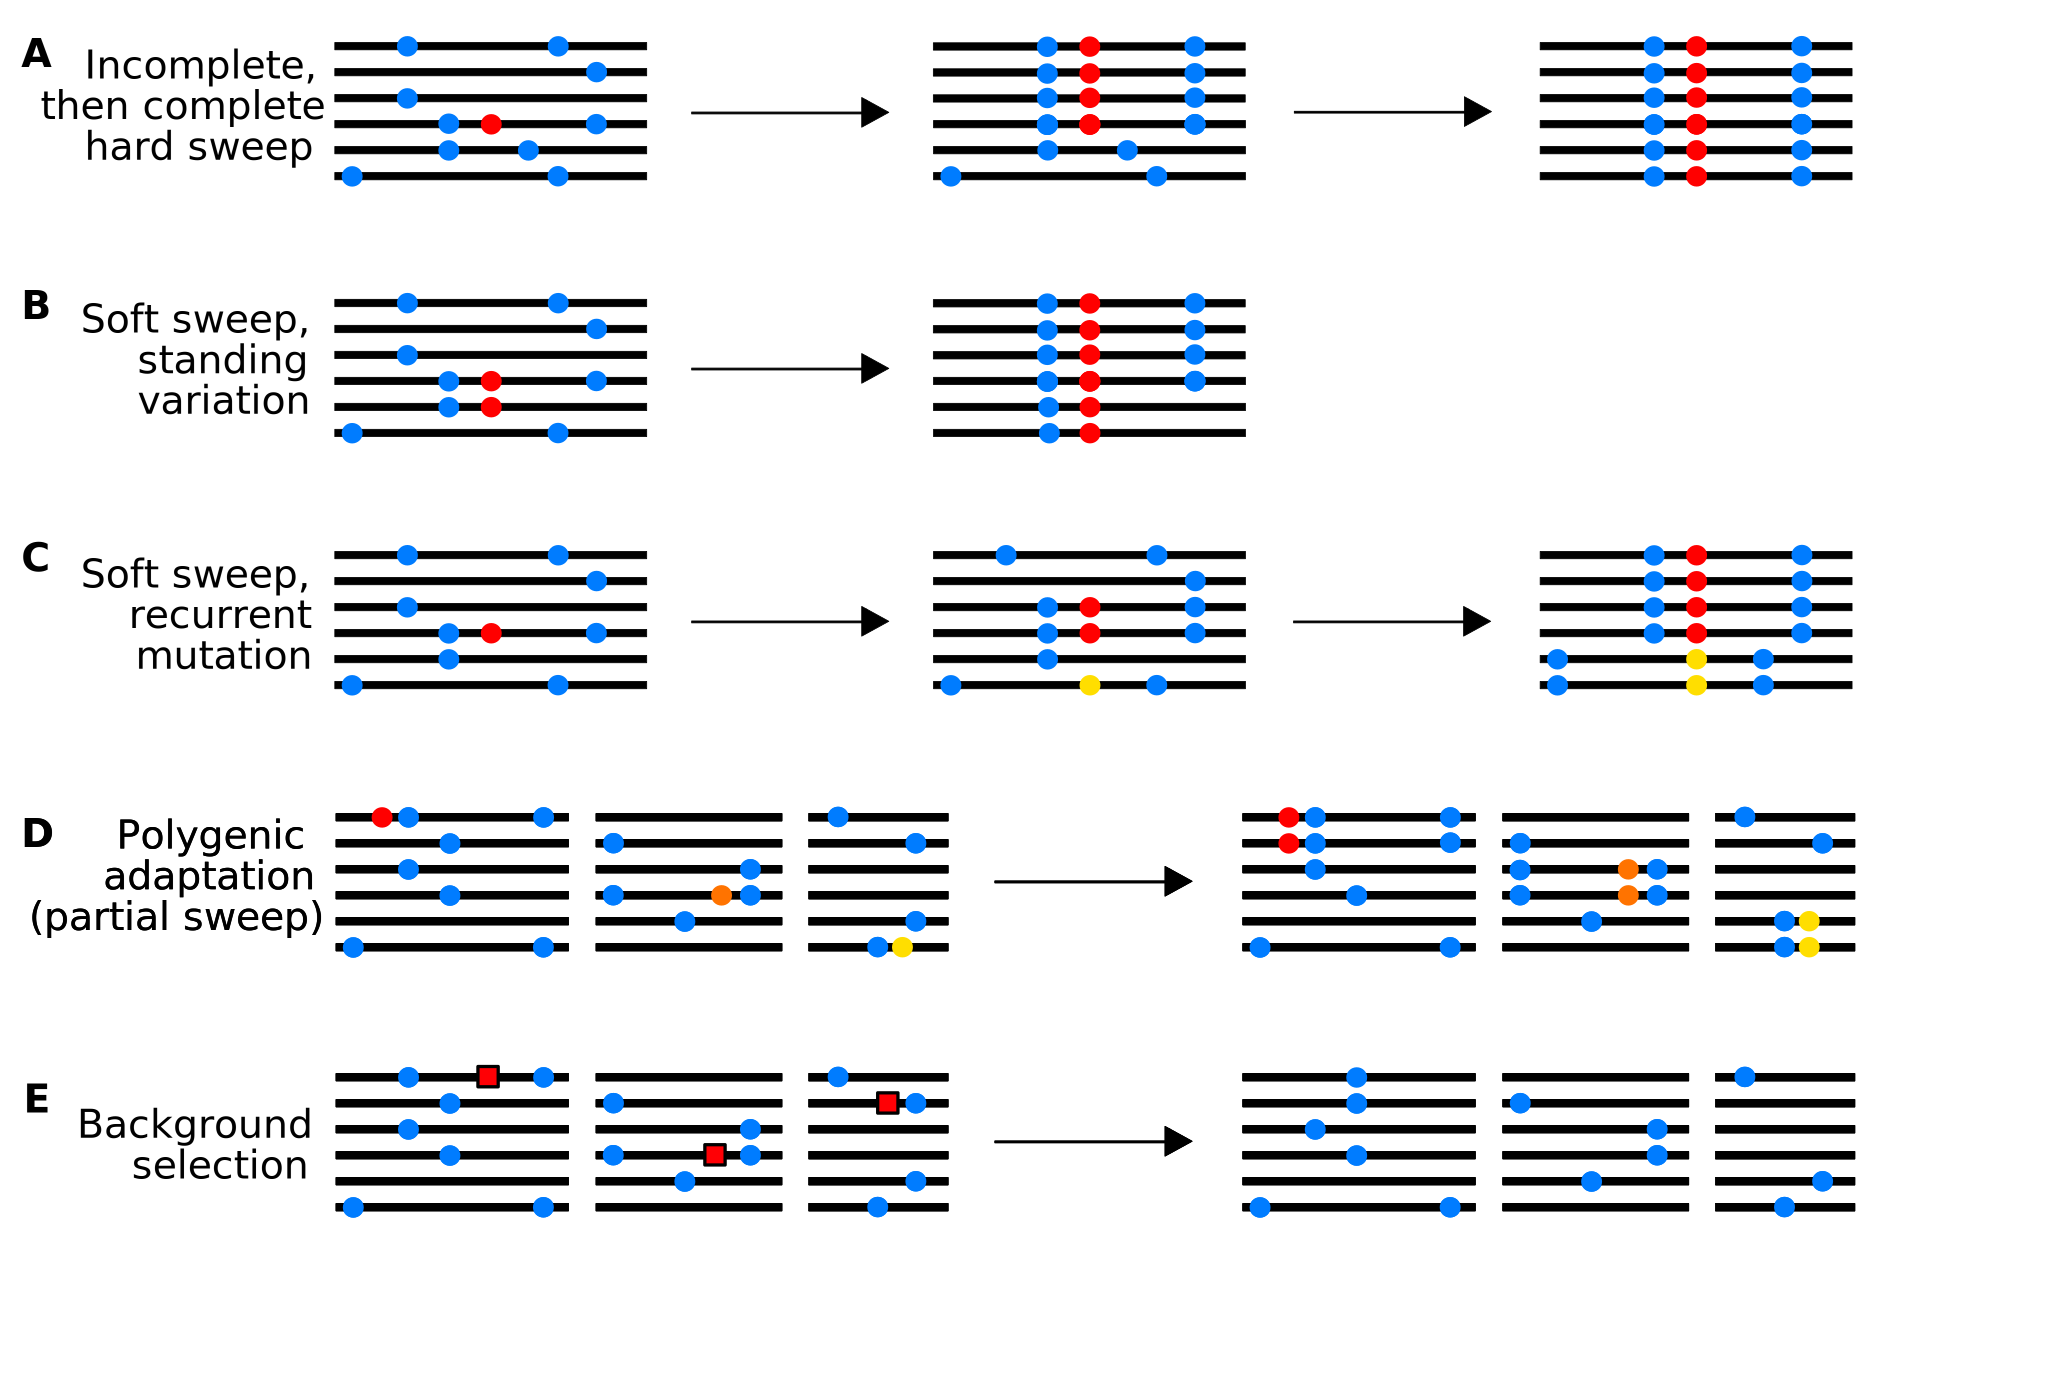
\includegraphics[width=\textwidth]{/Users/s0784966/Dropbox/Thesis/chapter1/figure_sweeps_no_legend.pdf}}
 \caption[Selective sweeps and background selection]{Selective sweeps and background selection. Blue circles are neutral varants, Reproduced from \cite{RN352}, thanks to Ben Jackson.}.
 
 \label{fig:sweepCartoon}
\end{figure}


\subsubsection{Hard/classic sweeps} 
 
The most well-studied model of sweeps. A new advantageous mutation rapidly increases in frequency to eventual fixation (shown in Figure \ref{fig:sweepCartoon}-A). As it sweeps, the adaptive allele carries with it a portion of the haplotype on which it arose, reducing levels of neutral diversity in the surrounding area \citep{RN124,RN235}. 
 
\subsubsection{Soft sweeps} 
  
A neutral allele segregating in a population may become favoured (due, for example, to a change in the environment). The segregating allele may be associated with multiple haplotypes, and as it rises in frequency, so do the multiple haplotypes (shown in \ref{fig:sweepCartoon}-B). A similar process, also termed a soft sweep, can occur if an advantageous mutation arises by multiple, distinct mutation events (shown in \ref{fig:sweepCartoon}-C). 
 
\subsubsection{Incomplete/partial sweeps} 
 
If an advantageous allele increases in frequency, but does not reach fixation, there will still be some loss of linked neutral diversity. In this review we use the term incomplete sweeps to describe sweeps that are polymorphic at the time of sampling, but may (or may not) eventually reach fixation (shown in \ref{fig:sweepCartoon}-A). The term partial sweep describes the situation wherein a sweeping allele becomes effectively neutral at a certain frequency in its trajectory (shown in \ref{fig:sweepCartoon}-D). The magnitude of both processes on linked neutral diversity depend on the frequency reached by the sweeping allele when selection is ‘turned off’ or on the time of sampling \citep{RN226}. Partial sweeps may be common in cases of adaptation involving selection on quantitative traits \citep{RN147}. 



\section[Using models of selective sweeps to estimate positive selection parameters]{Using Models of Selective Sweeps to Estimate Positive Selection Parameters $^*$}
 
Population geneticists have long sought to understand the contribution of natural selection to molecular evolution. A variety of approaches have been proposed that use population genetic theory to quantify the rate and strength of positive selection acting in a species’ genome. In the following section, I discuss methods that use patterns of between-species nucleotide divergence and within-species diversity to estimate positive selection parameters from population genomic data. We also discuss recently proposed methods to detect positive selection from a population’s haplotype structure. The application of these tests has resulted in the detection of pervasive adaptive molecular evolution in multiple species.
 
If adaptive substitutions are common, selection is expected to leave footprints in genetic diversity at linked sites. In particular, as a positively selected mutation increases in frequency, it tends to reduce diversity at linked neutral loci. Theoretical analysis of this process, termed a selective sweep (\textit{see above}), has shown that the reduction in diversity at a linked neutral locus depends on the ratio of the strength of positive selection to the recombination rate. Thus, comparing diversity at multiple neutral loci linked to selected regions, in principle, should provide an indirect means for estimating parameters of positive selection.

If a population experiences recurrent selective sweeps, there are several patterns predicted by theory. Under recurrent hard selective sweeps, levels of genetic diversity are expected to be lower i) in regions of the genome with restricted recombination, ii) in regions experiencing many sweeps and iii) in the genomic regions surrounding the targets of selection themselves. Each of these of these predictions have been met in empirical studies, and each has been used to estimate parameters of positive selection.

\subsection[The correlation between diversity and the rate of recombination]{The Correlation Between Diversity and the Rate of Recombination $^*$}

In the late 1980s, evidence began to emerge suggesting that genetic polymorphism are less frequent in genomic regions experiencing restricted crossing-over \citep{RN225,RN282}. Soon after, \cite{RN114} showed that there is a positive correlation between nucleotide diversity and the rate of crossing-over in \emph{D. melanogaster}, a pattern subsequently observed in other eukaryotic species \citep{RN117}. Begun and Aquadro pointed out that the correlation is qualitatively consistent with the action of recurrent selective sweeps. \cite{RN277} formulated expressions, based on the correlation between nucleotide diversity and the rate of recombination, to estimate the compound parameter $\lambda 2N_{e}s$, where $\lambda$ is the rate of sweeps per base pair per generation, $N_e$ is the effective population size and $s$ is the selection coefficient. They applied their method to the data of \cite{RN114}, estimating $\lambda2N_{e}s$ = 5.37 x $10^{-8}$, but their method could not disentangle the individual parameters. More recently, \cite{RN226} performed a similar analysis in \emph{D. melanogaster} to explore the effects of partial sweeps on parameter estimates. They showed that when partial sweeps are common, the rate of adaptive evolution is underestimated if the hard sweep model is assumed.
 
The correlation between diversity recombination observed by \cite{RN114} can also be explained by background selection, the reduction in neutral diversity caused by the removal of linked deleterious mutations \citep{RN132}. The process of background selection is qualitatively similar to recurrent selective sweeps, since both processes reduce local genetic diversity \citep{RN110} and skew the SFS towards rare variants \citep{RN287,RN133}. Models of background selection envisage a neutral site linked to many functional sites at different distances, such that the effects of selection accumulate to reduce diversity \citep{RN206, RN157}. The correlation between neutral diversity and the recombination rate predicted by background selection is quantitatively similar to that observed in \emph{D. melanogaster} \citep{RN281}. Indeed, recent studies suggest that background selection is a major determinant of nucleotide diversity variation at broad scales ($>$100Kbp) in humans \cite{RN120} and \emph{D. melanogaster} \citep{RN288, RN116}. It is clear, then, that background selection is a key confounding factor when attempting to make inferences about positive selection.
 
\subsection[Correlations between neutral diversity and non-neutral divergence]{Correlation Between Neutral Diversity and Non-Neutral Divergence $^*$}

If there is a constant fraction of adaptive substitutions, $\alpha$, across the genome for a given class of sites, regions that evolve at higher rates should experience a greater number of selective sweeps. Under a model of recurrent sweeps, it follows that there should be a negative correlation between nucleotide divergence at selected sites and diversity at linked neutral sites. This was first described in \textit{Drosophila melanogaster} by \cite{RN283}, and has been subsequently reported in other \textit{Drosophila} species \citep{RN284}. Assuming a single rate of sweeps ($\lambda$) and a constant scaled strength of positive selection ($2N_es$) for a given class of sites, \cite{RN283} generalised formulae of \cite{RN277} based on the correlation between synonymous site diversity and non-synonymous site divergence to estimate  $\lambda 2N_es$ = $3 \times 10^{-8}$ for the X-chromosome in \textit{D. melanogaster}. Note that this $\lambda 2N_es$ estimate is similar to that obtained based on the correlation of synonymous site diversity and recombination rate (\cite*{RN277}; see above). Using an estimate of $\alpha = 0.50$ obtained from a MK-based analysis, \cite{RN283} decomposed the $\lambda 2N_es$ compound parameter, and inferred that $s \approx 0.001\%$ and $\lambda$ = $3.6 x 10^{-11}$ /bp/generation, suggesting that adaptation of protein-coding genes in \textit{D. melanogaster} is driven by moderately weak selection (i.e., assuming \textit{D. melanogaster} $N_e =10^6$, $2N_es \approx 40$). In a related study, \cite{RN289} estimated $\lambda 2N_es \approx 10^{-7}$ in \textit{D. simulans}, also by examining the correlation between mean neutral diversity and selected (nonsynonymous) divergence. However, their model also included the heterogeneity in levels of diversity, which is related to the rate and strength of sweeps in a different way to the mean, and allowed the individual parameters to be fitted by regression. The estimates of the compound parameter $\lambda 2N_es$ are similar between the two studies, though \cite{RN289} estimated that $s \approx 1\%$ (compared to Andolfatto’s estimate of $s \approx 0.001 \%$) and $\lambda = 3.6 \times 10^{-12}$ /bp/generation. The discrepancies between the studies may be due to differences in biology between the species, or may reflect methodological differences: For example, if the majority of adaptive substitutions are driven by weakly selected sweeps, which will leave a relatively small signal in levels of  polymorphism, the MK-based method may more sensitively detect them, perhaps explaining the higher rate of sweeps inferred by \cite{RN283}. On the other hand, strongly selected sweeps will leave a larger footprint in levels of diversity, so will be more readily detected using the approach of \cite{RN289}, perhaps explaining why they inferred a lower overall rate of sweeps, with higher selection coefficients (for a full description, see \citealt{RN171}). In both cases, inferences based on variation in polymorphism may reflect processes other than the fixation of adaptive alleles that have gone to fixation, such as partial sweeps and background selection, as these will affect patterns of diversity but not necessarily divergence. Related to this, the approach employed by \cite{RN283} has recently been extended by \cite{RN323}, by estimating the correlation between synonymous site diversity and non-synonymous divergence in the presence of both background selection and gene conversion in \textit{D. melanogaster}. They found that ignoring background selection tends to increase and decrease estimates of selection strength and rate, respectively. The parameter values estimated in their study suggest that 0.02\% of new mutations at nonsynonymous sites are strongly selected ($s \approx 0.03\%$, assuming $N_e$ = $10^6$ for \textit{D. melanogaster}).
 
\subsection[Patterns of diversity around the targets of selection]{Patterns of Diversity Around the Targets of Selection $^*$}
 
An individual hard selective sweep is expected to leave a trough in genetic diversity around the selected site. If a large proportion of amino acid substitutions are adaptive, as suggested by MK-type analyses (see \citealt{RN215}), collating patterns of diversity around all substitutions of a given type should reveal a trough in diversity. Such a pattern is not expected around a “control” class of sites, such as synonymous sites. This test, proposed by \cite{RN167}, was first applied it to \textit{D. simulans}, and the above pattern was found. By fitting a hard sweeps model to the shape of the diversity trough, they estimated α values of  5\% and 13\%, depending on whether one or two classes of beneficial mutational effects were fitted. Note that their estimates of α are substantially lower than those obtained using MK-based methods for \textit{D. melanogaster} \citealt{RN283}. \cite{RN167} suggested that modes of selection other than hard sweeps may help explain to this discrepancy. However, even when modelling two classes of beneficial mutations, they found that amino acid substitutions are driven by strongly adaptive mutations ($s$ $sim0.5\%$ and $s$ $\sim0.01\%$). Their estimates of selection strength are therefore in broad agreement with the estimate of s $sim1\%$ obtained by \cite{RN289}, based on the correlation between synonymous diversity and non-synonymous divergence in \textit{D. simulans}. The \cite{RN167} test, then, suggests that adaptation in protein-coding genes is fairly frequent and driven by strong, hard sweeps.
 
The Sattath test has been applied in a variety of organisms, including humans \citep{RN162}, wild mice \citep{RN122}, \textit{Capsella grandiflora} \citep{RN236} and maize \citep{RN230}. In all but \textit{C. grandiflora}, researchers have found no difference in patterns of diversity around selected and neutral substitutions. These results have been interpreted as evidence that hard sweeps were rare in the recent history of both humans \citep{RN162} and maize \citep{RN230}. However, \cite{RN237} pointed out that the Sattath test will be underpowered if there is large variation in levels of functional constraint in the genome. Indeed, through their analyses \cite{RN237} found evidence for frequent adaptive substitutions in humans, particularly in regulatory sequence. To address the issues raised by \cite{RN237}, \cite{RN230} applied the Sattath test to substitutions in maize genes with the highest and lowest levels of functional constraint separately, but still found no difference in diversity pattern, suggesting either that hard sweeps have been rare in that species or that there is another confounding factor.
 
One possible explanation is that the species in which the Sattath test did/did not detect hard sweeps have distinct patterns of linkage disequilibrium (LD). LD decays to background levels within hundreds of base-pairs in \textit{D. simulans} \citep{RN283} and \textit{C. grandiflora} \citep{RN271}, whereas in humans, maize and wild mice it decays over distances closer to 10,000bp \citep{RN273,RN327, RN272}. It may be, then, that the Sattath test is only applicable when there is relatively short-range LD, such that the patterns of diversity around selected substitutions do not substantially overlap with the analysis windows around neutral ones. If this were the case, interpreting the similarity in troughs of diversity around selected and neutral substitutions as evidence for a paucity of hard selective sweeps may not be justified in organisms where LD decays over distances of a similar order of magnitude as the width of the diversity troughs themselves.
   	        	  
\section[Fitting genome wide patterns]{Fitting genome wide patterns $^*$}

	Methods to estimate the rate and strength of positive selection in the genome employ various combinations of nucleotide diversity, divergence, recombination rates and estimates of background selection effects as summary statistics, averaged over many regions of the genome. Recently, \cite{RN274} developed a method that fits a model of hard sweeps and background selection to genome-wide variation in nucleotide diversity and divergence (at both selected and neutral sites). In \textit{D. melanogaster}, they showed that hard sweeps can explain a large amount of genome-wide variation genetic diversity. For nonsynonymous sites, they found that $\alpha = 4.1\%$ for strongly selected mutations ($s \geq 0.03\%$) and $\alpha = 36.3\%$ for weakly selected mutations ($s \approx 0.0003\%$), summing to $\alpha = 40.4\%$, which is similar to the estimate obtained using the MK-test \citep{RN283}. Their results suggest that accounting for weakly selected mutations may help reconcile the discrepancy between MK-based estimates of the rate and strength of selection and parameters estimated from sweep model predictions, described above.

\cite{RN274} showed that a map of the effects of hard sweeps and background selection is capable of explaining a large amount of the variation in diversity across the genome, further demonstrating that the action of natural selection is pervasive, at least in \textit{D. melanogaster}. However, their method overestimated the rate of deleterious mutations, which the authors attribute to the presence of modes of adaptation other than hard sweeps in \textit{D. melanogaster}. 

\section[\citealt{RN122}]{\citealt{RN122}}


	The research I have performed throughout my PhD carries on from the work of \cite{RN122}, it is fitting, therefore, to give a brief description of the key findings from their study.
	
	\cite{RN122} sequenced the genomes of 10 wild-caught \textit{Mus musculus castaneus} individuals, using high-throughput sequencing methods. They sequenced individuals to high coverage, using multiple libraries of Illumina paired-end reads. Based on an analysis of population structure, the individuals sequenced were thought to represent a single admixed group. \cite{RN122} extracted polymorphism data from genomic regions around both protein-coding exons and conserved non-coding elements (CNEs - which were inferred to be involved in gene regulation), and found dips (or troughs) in average diversity surrounding the elements themselves. As discussed above, they then applied the Sattath analysis to their data, but found that there was no difference in the average diversity around nonsynonymous/synonymous substitutions. \cite{RN122} modelled the contribution BGS made to the troughs in diversity around both protein-coding exons and CNEs using a population genetic model, but found that it could not fully explain the patterns of diversity that they had observed. Our understanding of the factors that shape nucleotide diversity across the mouse genome are, thus, somewhat unclear.

\section[Thesis aims]{Thesis aims}

	The aim of this thesis is to further our understanding of the factors that shape variation in genetic diversity across the mammalian genome using the house mouse as a model. Particularly, I focus on the contributions of background selection and selective sweeps to variation in genetic diversity across the mouse genome. 

	\begin{itemize}
	
	\item In Chapter 2, I leverage information from patterns of linkage disequilibrium across the mouse genome and construct recombination rate maps for the mouse genome. 
	
	\item In Chapter 3, I estimate the distribution of fitness effects both advantageous and deleterious mutations for multiple classes of sites in the mouse genome. I use these estimates to parametrise forward-in-time population genetic simulations. These simulations are then analysed to scrutinise the parameters of selection we inferred.
	
	\item In Chapter 4, I fit a model incorporating the effects of both selective sweeps and background selection to troughs in diversity around functional elements in mice. Using the parameters that provide the best fit to the data, I ask whether adaptation in protein-coding or  regulatory regions contributes most to fitness in mice.
	
	\end{itemize}


	% Boot up the Chapter 2: Recombination file
	\chapter{The recombination landscape in wild house mice inferred using population genomic data}
\chaptermark{Recombination in wild mice}

\emph{This chapter has been published as a paper in Genetics: \\CITATION\\That paper is reproduced here.}
\section{Abstract}
Characterizing variation in the rate of recombination across the genome is important for understanding many evolutionary processes. The landscape of recombination has been studied previously in the house mouse, \emph{Mus musculus}, and it is known that the different sub-species exhibit different suites of recombination hotspots. However, it is not established whether broad-scale variation in the rate of recombination is conserved between the sub-species or whether hotspots identified in laboratory strains reflect the diversity of hotspots locations in natural populations. In this study, we construct a fine-scale recombination map for the Eastern house mouse sub-species, \emph{M. m. castaneus}, using 10 individuals sampled from its ancestral range. We perform simulations to assess how accurately recombination rates are inferred considering phasing errors. We use a novel approach to quantify phase error, which we estimate to affect 0.5\% of heterozygous SNPs in our data. We use LDhelmet to construct recombination maps for each autosome. We find that the spatial distribution of recombination rate is strongly positively correlated between our castaneus map and a map constructed using inbred lines of mice derived predominantly from \emph{M. m. domesticus}. However, despite this high similarity we find that potential recombination hotspots in wild mice show little overlap with the locations of double-strand breaks in wild-derived strains of laboratory mice, though the greatest overlap is with a strain derived from wild \emph{M. m. castaneus}. Finally, we also find that levels of genetic diversity in \emph{M. m. castaneus} are positively correlated with the rate of recombination, consistent with pervasive natural selection acting in the genome. Our study suggests that recombination rate variation is conserved at broad scales between two sub-species of \emph{M. musculus}, though not at fine scales.

\section{Introduction}
In many species, rates of crossing-over are not uniformly distributed across chromosomes, and understanding this variation and its causes is important for many aspects of molecular evolution. Experiments in laboratory strains or managed populations examining the inheritance of markers through pedigrees have allowed direct estimation of rates of crossing-over in different regions of the genome. Studies of this kind are impractical for many wild populations, where pedigree structures are largely unknown (but see Johnston et al. 2016). In mice, there have been multiple genetic maps published (e.g. Jensen-Seaman et al. 2004; Paigen et al. 2008; Cox et al. 2009; Liu et al. 2014), typically using the classical inbred laboratory strains, which are predominantly derived from the Western European house mouse sub-species, \emph{Mus musculus domesticus} (Yang et al. 2011). Recombination rate variation in laboratory strains may not, therefore, reflect natural rates and patterns in wild mice of different sub-species. In addition, recombination rate modifiers may have become fixed in the process of laboratory strain management. On the other hand, directly estimating recombination rates in wild house mice is not feasible without both a population’s pedigree and many genotyped individuals (but see Wang et al. 2017). 
 
        	To understand variation in recombination rates, patterns of linkage disequilibrium (LD) in a sample of individuals drawn from a population can be used. Coalescent-based methods have been developed that use such data to indirectly estimate recombination rates at very fine scales (Hudson 2001; Mcvean et al. 2002; Mcvean et al. 2004; Auton and Mcvean 2007; Chan et al. 2012). The recombination rates estimated in this way reflect variation in crossing-over rates in populations ancestral to the extant population, and are averages between the sexes. Methods using LD have been applied to explore variation in recombination rates among mammals and other eukaryotes, and have demonstrated that recombination hotspots are associated with specific genomic features (Myers et al. 2010; Paigen and Petkov 2010; Singhal et al. 2015).

The underlying mechanisms explaining the locations of recombination events have been the focus of much research. In house mice and in most other mammals, the PRDM9 zinc-finger protein binds to specific DNA motifs, resulting in an increased probability of double-strand breaks (DSBs), which can then be resolved by reciprocal crossing-over (Grey et al. 2011; Baudat et al. 2013). Accordingly, it has been shown that recombination hotspots are enriched for PRDM9 binding sites (Myers et al. 2010; Brunschwig et al. 2012). PRDM9-knockout mice still exhibit hotspots, but in dramatically different genomic regions (Brick et al. 2012). Variation in PRDM9, specifically in the exon encoding the zinc-finger array, results in different binding motifs (Baudat et al. 2010). Davies et al. (2016) generated a line of mice in which the exon encoding the portion of the PRDM9 protein specifying the DNA binding motif was replaced with the orthologous human sequence. The recombination hotspots they observed in this ‘humanized’ line of mice were enriched for the PRDM9 binding motif observed in humans. 

Great ape species have different alleles of the PRDM9 gene (Schwartz et al. 2014) and relatively little hotspot sharing (Winckler et al. 2005; Stevison et al. 2015). Correlations between the broad-scale recombination landscapes of the great apes are, however, relatively strongly positive (Stevison et al. 2011; Stevison et al. 2015). This suggests that, while hotspots evolve rapidly, the overall genetic map changes more slowly. Indeed, multiple closely related species pairs with different hotspot locations show correlations between recombination rates at broad scales (Smukowski and Noor 2011), as do species that share hotspots or lack them altogether (Singhal et al. 2015; Smukowski Heil et al. 2015).
 
It has been suggested that a population ancestral to the \emph{M. musculus} sub-species complex began to split into the present-day sub-species around 350,000 years ago (Geraldes et al. 2011). In this time, functionally distinct alleles of the PRDM9 gene and different suites of hotspots have evolved in the sub-species (Smagulova et al. 2016). In addition, between members of the \emph{M. musculus} sub-species complex, there is also variation in recombination rates at relatively broad scales for multiple regions of the genome (Dumont et al. 2011), and recombination rates can be polymorphic between \emph{M. m. domesticus} individuals (Wang et al. 2017). Brunschwig et al. (2012) analyzed single nucleotide polymorphism (SNP) data for classical laboratory strains of mice, and used an LD-based approach to estimate the sex-averaged recombination landscape for the 19 mouse autosomes. The recombination rate map they constructed is similar to a genetic map generated using crosses by Cox et al. (2009). Both studies were conducted using the classical inbred lines, whose ancestry is largely \emph{M. m. domesticus} (Yang et al. 2011), and their estimated recombination rate landscapes may therefore reflect that of \emph{M. m. domesticus} more than other members of the \emph{M. musculus} sub-species complex.
 
In this study, we construct a recombination map for the house mouse sub-species \emph{M. m. castaneus}. We used the genome sequences of 10 wild-caught individuals of \emph{M. m. castaneus} from the species’ expected ancestral range, originally reported by Halligan et al. (2013). In our analysis, we first phased SNPs and estimated rates of error in phasing. Secondly, we simulated data to assess the power of estimating recombination rates based on 10 individuals and the extent by which phase errors lead to biased estimates of the rate of recombination. Finally, using an LD-based approach, we inferred a sex-averaged map of recombination rates and compared this to previously published genetic maps for M. musculus. We show that variation in recombination rates in \emph{M. m. castaneus} is very similar to rate variation estimated in the classical inbred strains, at broad scales. However, we find little correspondence in fine-scale recombination rate variation between \emph{M. m. castaneus} and previously reported rate This suggests that, at broad scales, recombination rates have been relatively highly conserved since the sub-species began to diverge.

\section{Materials and Methods}

\subsection{Polymorphism data for \emph{Mus musculus castaneus}}
 
        	We analyzed the genomes of 10 wild-caught \emph{M. m. castaneus} individuals sequenced by Halligan et al. (2013). Samples were from North-West India, a region that is believed to be within the ancestral range of the house mouse. Mice from this region have among the highest levels of genetic diversity among the M. musculus sub-species (Baines and Harr 2007). In addition, the individuals sequenced represent a single population cluster and showed little evidence for substantial inbreeding (Halligan et al. 2010). Halligan et al. (2013) sequenced individual genomes to high coverage using multiple libraries of Illumina paired-end reads, which were mapped to the mm9 reference genome using BWA (Li and Durbin 2009). Mean coverage was >20x and the proportion of the genome with >10x coverage was more than 80\% for all individuals sampled (Halligan et al. 2013). Variants were called with the Samtools mpileup function (Li et al. 2009) using an allele frequency spectrum (AFS) prior. The AFS was obtained by iteratively calling variants until the spectrum converged. After the first iteration, all SNPs at frequencies >0.5 were swapped into the mm9 genome to construct a reference genome for \emph{M. m. castaneus}, which was used for subsequent variant calling (for further details see Halligan et al. 2013). The variant call format files generated by Halligan et al. (2013) were used in this study. In addition, alignments of \emph{Mus famulus} and \emph{Rattus norvegicus} to the mm9 genome, also generated by Halligan et al. (2013), were used as outgroups.
 
        	For the purposes of estimating recombination rates, variable sites were filtered on the basis of several conditions: Insertion/deletion polymorphisms were excluded, because the method used to phase variants (see below) cannot process these sites. We also excluded sites with more than two alleles and those that failed the Samtools Hardy-Weinberg equilibrium test (\emph{p} < 0.002).
 
\subsection{Inferring phase and estimating switch error rates}
 
LDhelmet estimates recombination rates from a sample of phased chromosomes or haplotypes drawn from a population. To estimate haplotypes, heterozygous SNPs called in \emph{M. m. castaneus} were phased using read-aware phasing in ShapeIt2 (Delaneau et al. 2013). ShapeIt2 uses sequencing reads that span multiple heterozygous variants, phase-informative reads (PIRs), and LD to phase variants at the level of whole chromosomes. Incorrectly phased heterozygous SNPs, termed switch errors, may upwardly bias estimates of the recombination rate, because they appear identical to legitimate crossing-over events. To assess the impact of incorrect phasing on our recombination rate inferences, we quantified the switch error rate as follows. The population sample of \emph{M. m. castaneus} comprised of seven females and three males. The X-chromosome variants in males therefore represent perfectly phased haplotypes. We merged the BAM alignments of short reads for the X-chromosome of the three males (samples H12, H28 and H34 from Halligan et al. (2013)) to make three datasets of pseudo-females, which are female-like, but in which the true haplotypes are known (H12+H28 = H40; H12+H34 = H46; H28 + H34 = H62). We then jointly re-called variants in the seven female samples plus the three pseudo-females using an identical pipeline as used by Halligan et al. (2013), as outlined above, using the same AFS prior.
 
Switch error rates in Shapeit2 are sensitive both to coverage and quality (per genotype and per variant) (Delaneau et al. 2013). We explored the effects of different filter parameters on the switch error rates produced by ShapeIt2 using the X-chromosomes of the pseudo-females. We filtered SNPs based on combinations of variant and genotype quality scores (QUAL and GQ, respectively) and on an individual’s sequencing depth (DP) (Table S1). For the individual-specific statistics (DP and GQ), if a single individual failed a particular filter, then that SNP was not included in further analyses. By comparing the known X-chromosome haplotypes and those inferred by ShapeIt2, we calculated switch error rates as the ratio of incorrectly resolved heterozygous SNPs to the total number of heterozygous SNPs for each pseudo-female individual. We used these results to choose filter parameters to apply to the autosomal data that generated a low switch error rate in ShapeIt2, while maintaining a high number of heterozygous SNPs. We obtained 20 phased haplotypes for each of the 19 mouse autosomes. With these, we estimated the recombination rate landscape for \emph{M. m. castaneus}.
 
\subsection{Estimating recombination maps and validation of the approach}
 
        	LDhelmet (v1.7; Chan et al. 2012) generates a sex-averaged map of recombination rates from a sample of haplotypes that are assumed to be drawn from a randomly mating population. Briefly, LDhelmet examines patterns of LD in a sample of phased chromosomal regions and uses a composite likelihood approach to infer recombination rates that are best supported between adjacent SNPs. LDhelmet appears to perform well for species with large effective population size ($N_e$) and has been shown to be robust to the effects of selective sweeps, which may be prevalent and reduce diversity in and around functional elements of the \emph{M. m. castaneus} genome (Halligan et al. 2013). The underlying model of LDhelmet relies on the assumption that populations are at recombination-drift equilibrium. We assume this to be the case for our sampled population, however violation of this may result in biased recombination rate estimates. However, the analyses conducted by Chan et al. (2012), in which the software was tested, were performed with a larger number of haplotypes than we have in our sample. To assess whether our smaller sample size gives reliable recombination maps, we validated and parameterized LDhelmet using simulated datasets.
 
        	A key parameter in LDhelmet is the block penalty, which determines the extent by which likelihood is penalized by spatial variation in the recombination rate, such that a high block penalty results in a smoother recombination map. We performed simulations to determine the block penalty that leads to the most accurate estimates of the recombination rate in chromosomes that have levels of diversity and base content similar to \emph{M. m. castaneus}. Chromosomes with constant values of $\rho$ = $4N_{e}r$ ranging from 2 x $10^{-6}$ to 2 x $10^1$ were simulated in SLiM v1.8 (Messer 2013). For each value of $\rho$, 0.5Mbp of neutrally evolving sequence was simulated for populations of \emph{N} = 1,000 diploid individuals. Mutation rates in the simulations were set using the compound parameter $\theta$ = $4N_{e}\mu$, where $\mu$ is the per-base, per-generation mutation rate. The mutation and recombination rates of the simulations were scaled to $\theta/4N$ and $\rho/4N$, respectively. $\theta$ was set to 0.01 for all simulations, as this is close to the genome-wide average for our data, based on pairwise differences. Simulations were run for 10,000 generations to achieve equilibrium levels of polymorphism, at which time 10 diploid individuals were sampled from the population. Each simulation was repeated 20 times, resulting in 10Mbp of sequence for each value of ρ. The SLiM output files were converted to sequence data, suitable for analysis by LDhelmet, using a custom Python script that incorporated the mutation rate matrix estimated for non-CpG prone sites in \emph{M. m. castaneus} (see below). We inferred recombination rates from the simulated data in windows of 4,400 SNPs with a 200 SNP overlap between windows, following (Chan et al. 2012). We analyzed the simulated data using LDhelmet with block penalties of 10, 25, 50 and 100. The default parameters of LDhelmet are tuned to analyze \emph{Drosophila melanogaster} data (Chan et al. 2012). Since the \emph{D. melanogaster} population studied by Chan et al. (2012) has comparable levels of genetic diversity to \emph{M. m. castaneus} we used the defaults for all other parameters, other than the block penalty and estimate of $\theta$.
 
        	Errors in phase inference, discussed above, may bias our estimates of the recombination rate, since they appear to break apart patterns of LD. We assessed the impact of these errors on recombination rate inference by incorporating them into the simulated data at a rate estimated from the pseudo-female individuals. For each of the 10 individuals drawn from the simulated populations, switch errors were randomly introduced at heterozygous positions at the rate estimated using the chosen SNP filter set (see Results). We then inferred the recombination rates, as above, for the simulated population using these error-prone data. We assessed the effect of switch errors on recombination rate inference by comparing estimates based on the simulated data both with and without switch errors. It is worth noting that there is the potential for switch errors to undo crossing-over events, reducing inferred recombination rates, if they affect heterozygous SNPs that are breakpoints of recombinant regions. 

\subsection{Recombination rate estimation for \emph{M. m. castaneus}}
        	
        We used LDhelmet (Chan et al. 2012), to estimate recombination rates for each of the \emph{M. m. castaneus} autosomes. It is well established that autosomal recombination rates differ between the sexes in \emph{M. musculus} (Cox et al. 2009; Liu et al. 2014). A drawback of LD-based approaches is that they give sex-averaged recombination rates. 
 
        	We used both \emph{M. famulus} and \emph{R. norvegicus} as outgroups to assign ancestral alleles to polymorphic sites. LDhelmet incorporates both the mutation matrix and a prior probability on the ancestral allele at each variable position as parameters in the model. We obtained these parameters as follows. For non-CpG prone polymorphic sites, if the outgroups shared the same allele, we assigned that allele as ancestral and these sites were then used to populate the mutation matrix, following Chan et al. (2012). This approach ignores the possibility of both back mutation and homoplasy. To account for this uncertainty, LDhelmet incorporates a prior probability on the ancestral base. Following Singhal et al. (2015), at resolvable sites (i.e. when both outgroups agreed), the ancestral base was given a prior probability of 0.91, with 0.03 assigned to each of the three remaining bases. This was done to provide high confidence in the ancestral allele, but to also include the possibility of ancestral allele misinference. At unresolved sites (i.e., if the outgroup alleles did not agree or there were alignment gaps in either outgroup), we used the stationary distribution of allele frequencies from the mutation rate matrix as the prior (Table S2).
 
We analyzed a total of 44,835,801 SNPs in LDhelmet to construct recombination maps for each of the \emph{M. m. castaneus} autosomes and the X-chromosome. Following Chan et al. (2012), windows of 4,400 SNPs, overlapping by 200 SNPs on either side, were analysed. We ran LDhelmet for a total of 1,000,000 iterations, discarding the first 100,000 as burn-in. A block penalty of 100 was chosen to obtain a conservatively estimated broad-scale recombination map. For the purposes of identifying recombination hotspots, we re-ran the LDhelmet analysis with a block penalty of 10. We analyzed all sites that passed the filters chosen using the pseudo-female phasing analysis regardless of CpG status; note that excluding CpG-prone sites removes $\sim50\%$ of the available data and thus would substantially reduce the power to infer recombination rates. We assumed $\theta$ = 0.01, the approximate genome-wide level of neutral diversity in \emph{M. m. castaneus}, and included ancestral allele priors and the mutation rate matrix for non-CpG sites as parameters in the model. Following the analyses, we removed overlapping SNPs and concatenated SNP windows to obtain recombination maps for whole chromosomes. 

It is worthwhile noting that our recombination maps were constructed with genotype calls made using the mm9 version of the mouse reference genome. This version was released in 2007 and there have been subsequent versions released since then. However, previously published genetic maps for M. musculus were constructed using mm9, so we used that reference to make comparisons (see below).
 
\subsection{Broad scale comparison to previously published maps}
 
The recombination rate map inferred with a block penalty of 100 for \emph{M. m. castaneus} was compared with two previously published genetic maps for M. musculus. The first map was generated by analyzing the inheritance patterns of markers in crosses between inbred lines (Cox et al. 2009) (downloaded from http://cgd.jax.org/mousemapconverter/). Hereafter, this map shall be referred to as the Cox map. The second map was generated by Brunschwig et al. (2012), by analyzing SNPs in classical inbred mouse lines using LDhat (Auton and Mcvean 2007), the software upon which LDhelmet is based (available at http://www.genetics.org/content/early/2012/05/04/genetics.112.141036). Hereafter, this map shall be referred to as the Brunschwig map. Both the Brunschwig and Cox maps were constructed using far fewer markers than the present study, $\sim500,000$ and $\sim10,000$ SNPs, respectively and both maps were generated using classical strains of laboratory mice, which are predominantly of \emph{M. m. domesticus} origin (Yang et al. 2011). For example, in the classical inbred strains analyzed by Cox et al. (2009), the mean genome-wide ancestry attributable to \emph{M. m. domesticus}, \emph{M. m. musculus} and \emph{M. m. castaneus} is 94.8\%, 5.0\% and 0.2\%, respectively (data downloaded from the Mouse Phylogeny Viewer (Wang et al. 2012) http://msub.csbio.unc.edu). Values for all classical strains, 60 of which were analyzed by Brunschwig et al. (2012), are similar (Yang et al. 2011).

Recombination rates in the Brunschwig map and our castaneus map were inferred in terms of the population recombination rate ($\rho$ = 4Ner), units that are not directly convertible to centimorgans (cM), but were converted to cM/Mb for comparison purposes using frequency weighted means, as follows. Both LDhat and LDhelmet give estimates of $\rho$ (per Kbp and bp, respectively) between pairs of adjacent SNPs. To account for differences in the physical distance between adjacent SNPs when calculating cumulative $\rho$, we used the number of bases between a pair of SNPs to weight that pair’s contribution to the sum. By setting the total map distance for each chromosome to be equal to those found by Cox et al. (2009), we scaled the cumulative ρ at each analyzed SNP position to cM values.
 
At the level of whole chromosomes, we compared mean recombination rates from the castaneus map with several previously published maps. The frequency-weighted mean recombination rates (in terms of $\rho$) for each of the chromosomes from the castaneus and Brunschwig maps were compared with the cM/Mb values obtained by Cox et al. (2009) as well as independent estimates of the per chromosome recombination rates from Jensen-Seaman et al. (2004). Pearson correlations were calculated for each comparison. Population structure in the inbred line data analyzed by Brunschwig et al. (2012) may have elevated LD, thus downwardly biasing estimates of $\rho$. To investigate this, we divided the frequency-weighted mean recombination rates per chromosome from the castaneus and Brunschwig maps by the rates given in Cox et al. (2009) to obtain estimates of effective population size.
 
At the Mbp scale, we compared variation in recombination rates across the autosomes in the different maps using windows. We calculated Pearson correlations between the frequency weighted-mean recombination rates (in cM/Mb) in non-overlapping windows for the castaneus, Cox and Brunschwig maps. The window size considered may affect the correlation between maps, so we calculate Pearson correlations in windows of 1Mbp to 20Mbp in size. For visual comparison of the castaneus and Cox maps, we plotted recombination rates in sliding windows of 10Mbp, offset by 1Mb. 

\subsection{Fine-scale recombination rate variation in wild \emph{M. m. castaneus}}

To assess the distribution of fine-scale recombination rates in \emph{M. m. castaneus} we used Gini coefficients and Lorenz curves. Applied to genetic maps, Gini coefficients and Lorenz curves have been used as a quantitative measure of the extent of heterogeneity of recombination rates in a genome (e.g. Kaur and Rockman 2014). Using our recombination maps generated using a block penalty of 10, we constructed Lorenz curves and calculated their Gini coefficients for each chromosome separately.

	Recombination hotspots can be operationally defined as small windows of the genome that exhibit elevated rates of recombination relative to surrounding regions. To obtain the locations of potential recombination hotspots we adapted a script used by Singhal et al. (2016). We divided the genome into non-overlapping windows 2Kbp wide and, using the maps we generated using a block penalty of 10, classified all windows where the recombination rate was at least 5x greater than the recombination rate in the surrounding 80Kbp as potential hotspots. After identification, we merged all hotspots that were located directly next to one another.

	To ask whether the fine-scale recombination rate variation in \emph{M. m. castaneus} is like that reported for inbred lines, we compared the locations of putative hotspots in our data to the locations of DSBs reported by Smagulova et al. (2016). In their study, Smagulova et al. (2016) generated sequencing reads corresponding to the locations of DSBs in inbred strains of mice representing each of the principle M. musculus sub-species as well as \emph{M. m. molossinus}, an inter-sub-specific hybrid of \emph{M. m. castaneus} and \emph{M. m. musculus}. Their reads were mapped to the mm10 genome so to compare the locations of we converted the coordinates of DSBs to mm9 using the UCSC LiftOver tool (https://genome.ucsc.edu/cgi-bin/hgLiftOver), using the default parameters. The locations of putative hotspots present in our dataset were compared to the locations of DSBs in each of the strains studied by Smagulova et al. (2016) using BedTools v2.17.0 (Quinlan and Hall 2010). To determine the amount of overlap between our list of hotspots and each of the lists of DSBs expected by chance, we approximated the null distribution of hotspot sharing using a randomization approach. For each of the inbred strains analyzed by Smagulova et al., we randomized the locations of our putative hotspots (using BedTools shuffle with the –chrom option) and obtained the number of overlapping hotspots and DSB locations. For each comparison, this procedure was repeated 1000 times, per inbred strain, and the maximum number of null overlaps was taken as an approximate 0.1\% significance threshold.
 
\subsection{Examining the correlation between nucleotide diversity and recombination rate}

There is evidence that natural selection is pervasive in the protein-coding genes and conserved non-coding elements in the murid genome (Halligan et al. 2010; Halligan et al. 2011; Halligan et al. 2013). Directional selection acting on selected sites within exons may reduce diversity at linked neutral sites through the processes of background selection and/or selective sweeps. These processes have the largest effect in regions of low recombination, and can therefore generate positive correlations between diversity and the recombination rate, as has been observed in multiple species (Cutter and Payseur 2013). We used our castaneus map to examine the relationship between nucleotide diversity and recombination rates as follows. We obtained the coordinates of the canonical spliceforms of protein coding genes, orthologous between mouse and rat from Ensembl Biomart (Ensembl Database 67; http://www.ensembl.org/info/website/archives/index.html). We calculated the frequency-weighted mean recombination rate, from the block penalty 100 map, and the GC content for each gene. Using the approximate castaneus reference, described above, and the outgroup alignment, we obtained the locations of 4-fold degenerate synonymous sites. If a site was annotated as 4-fold in all three species considered, it was used for further analysis. We removed poor quality alignments between mouse and rat, exhibiting a spurious excess of diverged sites, where > 80\% of sites were missing. We also excluded five genes that were diverged at all non-CpG prone 4-fold sites, as it is likely that these also represent incorrect alignments. After filtering, there were a total of 18,171 protein-coding genes for analysis.

We examined the correlation between local recombination rates in protein coding genes with nucleotide diversity and divergence. Variation in the mutation rate across the genome may influence genome-wide analyses of nucleotide polymorphism, so we also examined the correlation between the ratio of nucleotide diversity and divergence from R. norvegicus at neutral sites and the rate of recombination. We used non-parametric Kendall rank correlations for all comparisons.

All analyses were conducted using Python scripts, except correlation analyses which were conducted using R (R Core Team 2016) and hotspot identification which was done using a Python script adapted from one provided by Singhal et al. (2016). 

\section{Results}
 
\subsection{Phasing SNPs and estimating the switch error rate}
 
In order to infer recombination rates from our sample of individuals, we required phased SNPs. Taking advantage of the high sequencing depth of the sample generated by Halligan et al. (2013), we phased SNPs using ShapeIt2, an approach that makes use of both LD and sequencing reads to resolve haplotypes. We phased each of the mouse autosomes, giving a total of 44,835,801 SNPs for estimation of recombination rates (Table S3). 
 
By constructing pseudo-female individuals, we quantified the switch error rate incurred when inferring phase from our data. After filtering of variants, ShapeIt2 achieved low switch error rates for all parameter combinations tested (Table S1). We chose a set of filters (GQ > 15, QUAL > 30) that resulted in a mean switch error rates across the three pseudo-females of 0.46\% (Table S1) and filtered out, on average, 44\% of the available SNPs (Table S3). More stringent filtering resulted in slightly lower mean switch error rates, but also resulted in the removal of many more variants from the dataset (Table S1), thus reducing power to resolve recombination rates in downstream analyses.
 
\subsection{Simulations to validate LDhelmet for the population sample of \emph{M. m. castaneus}}
 
We assessed the performance of LDhelmet when applied to our dataset by simulation. In the absence of switch errors, LDhelmet accurately infers the average recombination rate down to values of $\rho/bp$ = 2 x $10^{-4}$ (Figure 1). Below this value, LDhelmet overestimated the scaled recombination rate for the simulated populations (Figure 1). With switch errors incorporated into simulated data, LDhelmet accurately estimated $\rho/bp$ in the range 2 x $10^{-3}$ to 2 x $10^{2}$. When the true $\rho/bp$ was $<$ 2 x $10^{-3}$, however, LDhelmet overestimated the mean recombination rate for 0.5Mbp regions (Figure 1). This behavior was consistent for all block penalties tested (Figure S1). Given that the simulations incorporated the mutation rate matrix (Table S2) and mutation rate ($\theta$ = $4N_{e}\mu$) estimated for \emph{M. m. castaneus} we concluded that LDhelmet is applicable to the dataset of 10 \emph{M. m. castaneus} individuals sequenced by Halligan et al. (2013).
 
 
 \begin{figure}[h]
   \centering      
   \noindent\makebox[\textwidth]{\includegraphics[width=\textwidth]{/Users/s0784966/Dropbox/Thesis/chapter2/Figures/Figure1.pdf}}
 \caption[The effect of switch errors on recombination rate inference]{The effect of switch errors on the mean recombination rate inferred using LDhelmet with a block penalty of 100. Each black point represents results for a window of 4000 SNPs, with 200 SNPs overlapping between adjacent windows, using sequences simulated in SLiM for a constant value of $\rho/bp$. Red points are mean values. Switch errors were randomly incorporated at heterozygous SNPs with probability 0.0046. The dotted line shows the value when the inferred and true rates are equal}
 \label{fig:1}
\end{figure}

\subsection{Recombination rates in the \emph{M. m. castaneus genome}}
 
A recombination rate map for each \emph{M. m. castaneus} autosome was constructed using LDhelmet. We analyzed a total of 44,835,801 phased SNPs across the 19 mouse autosomes and the X-chromosome. From the map constructed using a block penalty of 100, the frequency weighted mean value of $\rho/bp$ for all autosomes was 0.009. This value is greater than the lower detection limit suggested by both the simulations with and without switch errors (Figure 1). For the X-chromosome, the frequency-weighted mean rate was 0.0026, which is closer to the lower detection limit, but still above it (Figure 1). Because of this, the lower SNP density and smaller number of alleles used for inference, results for the X-chromosome may be more error-prone than for the autosomes. 

We assessed variation in whole-chromosome recombination rates between our LD-based castaneus map and direct estimates of recombination rates published in earlier studies. Comparing the mean recombination rates for whole chromosomes provides us with a baseline comparison for which we have an a priori expectation: We expect that chromosome 19, the shortest in physical length, should have the highest mean recombination rate since at least one crossing-over event is required per meiosis per chromosome in mice and that the X-chromosome, which only undergoes recombination in females, should have the lowest rate. Both expectations have been met in previous studies of recombination in \emph{M. musculus} (Jensen-Seaman et al. 2004; Cox et al. 2009). Indeed, we find that the frequency-weighted mean recombination rates for chromosome 19 and the X-chromosome are the highest and lowest, respectively (Table 1). We also found that the frequency-weighted mean recombination rates for each of the chromosomes we analyzed were highly correlated with the direct estimates given in Jensen-Seaman et al. (2004) (Pearson correlation = 0.59, \emph{p} = 0.005) and Cox et al. (2009) (Pearson correlation = 0.68, \emph{p} = 0.001), excluding the X-chromosomes does not substantially change the correlation results. These correlations suggest that our analysis captures real variation in recombination rates at the scale of whole chromosomes in the \emph{M. m. castaneus} genome. 

\begin{figure}[h]
   \centering      
   \noindent\makebox[\textwidth]{\includegraphics[width=\textwidth]{/Users/s0784966/Dropbox/Thesis/chapter2/Figures/Figure2.pdf}}
 \caption[Comparison of LD-based and pedigree-based recombination maps]{Comparison of sex-averaged recombination rates for chromosomes 1 and 19 of \emph{M. m. castaneus} inferred by LDhelmet (red) with rates estimated in the pedigree-based study of Cox et al. (2009) (blue). Recombination rates were scaled to units of centimorgans per megabase for the castaneus map by setting the total map length of each chromosome to the corresponding map length of Cox et al. (2009).}
\end{figure}

\linespread{1}

\begin{sidewaystable}
\caption[Summary of recombination rates per chromosomes]{Summary of sex-averaged recombination rates \emph{M. m castaneus} compared with the rates from Brunschwig et al. (2012) and Cox et al. (2009). Rates for the castaneus and Brunschwig maps are presented in terms of $4N_{e}r/bp$. Estimates of $N_e$ were obtained by assuming the recombination rates from Cox et al. (2009).}
 \begin{tabular}{c c c c c c} 
  \hline
 Chromosome & Cox cM/Mb & Freq. Weighted Mean & $N_e$ Estimate & Freq. Weighted Mean & $N_e$ Estimate \\ [0.5ex] 

 \hline
 1 & 0.50 & 0.0079 & 395,000 & 0.000015 & 745\\
 2 & 0.57 & 0.0088 & 386,000 & 0.000015 & 653\\
 3 & 0.52 & 0.0083 & 400,000 & 0.000014 & 693\\
 4 & 0.56 & 0.0091 & 408,000 & 0.000020 & 889\\
 5 & 0.59 & 0.0090 & 382,000 & 0.000015 & 646\\
 6 & 0.53 & 0.0089 & 421,000 & 0.000015 & 728\\
 7 & 0.58 & 0.0100 & 429,000 & 0.000019 & 801\\
 8 & 0.58 & 0.0094 & 404,000 & 0.000014 & 610\\
 9 & 0.61 & 0.0096 & 394,000 & 0.000018 & 749\\
 10 & 0.61 & 0.0096 & 392,000 & 0.000023 & 928\\
 11 & 0.70 & 0.0102 & 365,000 & 0.000019 & 689\\
 12 & 0.53 & 0.0089 & 420,000 & 0.000019 & 897\\
 13 & 0.56 & 0.0095 & 426,000 & 0.000014 & 629\\
 14 & 0.53 & 0.0084 & 395,000 & 0.000013 & 632\\
 15 & 0.56 & 0.0083 & 371,000 & 0.000024 & 1,080\\
 16 & 0.59 & 0.0091 & 386,000 & 0.000017 & 721\\
 17 & 0.65 & 0.0087 & 335,000 & 0.000052 & 2,020\\
 18 & 0.66 & 0.0098 & 371,000 & 0.000021 & 785\\
 19 & 0.94 & 0.0122 & 323,000 & 0.000026 & 681\\
 X & 0.48 & 0.0026 & 137,000 & - & -\\
 Mean & - & 0.0092 & - & 0.000020 &  -\\[1ex] 
 \hline
\end{tabular}    

\end{sidewaystable}


\linespread{2}


\subsection{Comparison of the \emph{M. m. castaneus} map to maps constructed using inbred lines}
 
We compared the intra-chromosomal variation in recombination rates between our castaneus map and previously published maps. Figure 2 shows the variation in recombination rates across the largest and smallest autosomes in the mouse genome, chromosomes 1 and 19, respectively. It is clear that the castaneus and Cox maps are very similar (see also Figure S2 showing a comparison of all autosomes). Correlation coefficients between the maps are $>$0.8 for window sizes of 8Mbp and above (Figure 3), though the correlations are noisier when considering chromosomes separately (Figure S3). Although the broad-scale correlation between the castaneus and Cox maps is high (Figure 3), there were several regions of the genome that substantially differ, for example in the center of chromosome 9 (Figure S2). The Cox and castaneus maps are more similar to one another than either are to the Brunschwig map (Figure 3). This is presumably because the Brunschwig map was constructed using an LD-based approach with a sample of 60 inbred mouse strains and a relatively low SNP density. Population structure in the lines used by Brunschwig et al. (2012) or the sub-species from which they were derived would elevate LD, resulting in downwardly-biased chromosome-wide values of $\rho$. This is also reflected in the $N_e$ values estimated from the frequency-weighted average recombination rates for each chromosome. The estimates of Ne are substantially different between the castaneus and Brunschwig maps, i.e. the castaneus estimates are consistently $\sim500\times$ higher (Table 1). The estimates of Ne from the castaneus map are in broad agreement with the estimates of Ne based on polymorphism data (Geraldes et al. 2008; Geraldes et al. 2011). The lower SNP density used to construct the Brunschwig map would also likely result in a lower resolution recombination map.

\linespread{1}
\begin{figure}[h]
   \centering      
   \noindent\makebox[\textwidth]{\includegraphics[width=\textwidth]{/Users/s0784966/Dropbox/Thesis/chapter2/Figures/Figure3.pdf}}
 \caption[Broad-scale correlations between recombiantion maps for \emph{Mus musculus castaneus} and \emph{Mus musculus domesticus}]{Pearson correlation coefficients between the recombination map inferred for \emph{M. m. castaneus}, the Brunschwig et al. (2012) map and the Cox et al. (2009) map. Correlations were calculated in nonoverlapping windows of varying size across all autosomes. Confidence intervals (95\%) are indicated by shading}
\end{figure}
\linespread{2}

\subsection{Analysis of fine-scale recombination rates in wild \emph{M. m. castaneus}}


To locate potential recombination hotspots in wild M. m. castaneus we ran LDhelmet at a lower block penalty. As expected, the lower block penalty introduced more fine-scale variation into the recombination map; for example, see Figure S4. We used this fine-scale variation to locate 39,972 potential recombination hotspots in wild M. m. castaneus across the autosomes and X-chromosome. On average, there was 15 hotspots per Mbp across for all chromosomes tested. The total number of putative hotspots we identified is more than double the 15,061 DSB locations identified for CAST, a wild-derived strain representing M. m. castaneus, by Smagulova et al. (2016). In classical inbred lines, a total of 47,073 recombination hotspots were previously identified using a coalescent-based approach by Brunschwig et al. (2012), though they did not analyze the X-chromosome in their study. 

To obtain a measure of the heterogeneity of recombination rates in the genome, we constructed Lorenz curves and calculated their Gini coefficients (Figure S5). In the context of a genetic map, Gini coefficients close to zero represent more uniform distributions of crossing-over rates and values closer to one indicates that recombination events are restricted to a small number of locations in a genome. Using the map constructed with a block penalty of 10, the mean Gini coefficient for across all autosomes was found to be 0.78. Our estimate is in line with that of Kaur and Rockman (2014), who reported a median Gini coefficient of 0.77 for chromosome 1 in inbred mice using a high-density map of crossing over locations observed in a crossing study (Paigen et al. 2008). The Lorenz curve for the X-chromosome was distinct from the autosomes (Figure X), however, with a Gini coefficient of 0.95, which is similar to the upper limit of the confidence interval around the estimate of Kaur and Rockman (2014). 

We compared the locations of our potential recombination hotspots to the positions of DSBs reported by Smagulova et al. (2016). We found only a small overlap between the locations of potential recombination hotspots inferred for wild-caught mice and the locations of DSBs observed in the wild-derived inbred strains analyzed by Smagulova et al. (2016) (Table S4). The inbred strain CAST, representing M. m. castaneus, had the greatest amount of overlap, with 12.2\% of DSB locations overlapping a putative hotspot and 4.1\% after correcting for the number of overlaps expected seen by chance (Table S4). The second greatest overlap was with PWD, a strain that represents \emph{M. m. musculus} (Table S4). All strains representing \emph{M. m. domesticus} (13R, B6 and C3H) showed less than 1\% overlap after correction. Note that our estimates of the null expectation are likely conservative, as false positives due to, for example, switch errors, present in our set of putative hotspots will inflate the probability of chance overlaps. 

\subsection{Correlations between recombination rate and properties of protein coding genes in \emph{M. m. castaneus}}

	By examining the correlation between genetic diversity and recombination rate, we determined whether our map captures variation in $N_e$ across the genome. We found that recombination rates at autosomal protein coding genes are significantly and positively correlated with levels of neutral genetic diversity, at all sites regardless of base context and at non-CpG-prone sites only (Table 2). Divergence from the rat at 4-fold sites was also significantly and positively correlated with recombination rate when analyzing all sites. However, for non-CpG-prone sites we found a small negative correlation (Table 2). There was also a significant and positive relationship between recombination rate and a gene’s GC content ($\tau$ = 0.125, p $<$ 2.2 x $10^{-16}$). The correlation between recombination rate and neutral diversity divided by divergence from the rat was both positive and significant, regardless of base context (Table 2; Figure S6). This indicates that natural selection may have a role in reducing diversity via hitchhiking and/or background selection.

\linespread{1}

\begin{table}[H]
\centering
\caption[Estimates of the DFE for three classes of functional sites]{Parameter estimates for the distribution of fitness effects for three classes of sites in \textit{M. m. castaneus} obtained under two models. The first (Model A) estimates of selection parameters based on the full uSFS. Under the second method (Model B), sites fixed for the derived allele were prevented from influencing estimates of selection parameters. The bracketed values are 95\% confidence intervals obtained from profile likelihoods. The parameters shown are: $p(i)$ = the proportion of mutations falling into the $i^{th}$ deleterious class; $2N_es(i)$ = the scaled homozygous selection coefficient of the $i^{th}$ deleterious class; $p_a$ = the proportion of advantageous mutations; $2N_es_a$ = the scaled homozygous selection coefficient of the advantageous mutation class.}

\begin{tabular}{cccc}
\toprule
          \multicolumn{4}{c}{\textbf{Model A: DFE inferred from the full uSFS}} \\
                  &     \textbf{0-fold} &        \textbf{UTR} &        \textbf{CNE} \\ \hline
                  $2N_es(1)$ &      -0.09 &     -0.194 &     -0.646 \\
                  $p(1)$ &      0.191 &      0.701 &      0.352 \\
                  $2N_es(2)$ &       -208 &      -78.2 &      -7.96 \\
                  $p(2)$ &      0.806 &      0.286 &      0.278 \\
                  $2N_es(3)$ &          - &          - &     -155.8 \\
                  $p(3)$ &          - &          - &       0.36 \\
                            &            &            &            \\
                  $2N_es_a$ &      14.54 &      10.64 &      18.34 \\
				            & [9.24 – 23.4] & [7.82 – 14.1] & [14.0 – 41.8] \\
                  $p_a$ &      0.003 &      0.013 &     0.0098 \\
							& [0.0019 – 0.0048] & [0.0097 – 0.019] & [0.0037 – 0.0099] \\ \midrule
\multicolumn{4}{c}{\textbf{Model B: Fixed derived alleles do not affect parameter estimates}}  \\ 
                  &     \textbf{0-fold} &        \textbf{UTR} &        \textbf{CNE} \\ \hline
                 $2N_es(1)$ &     -0.342 &      -0.32 &     -0.506 \\
                 $p(1)$ &      0.184 &      0.689 &      0.342 \\
                 $2N_es(2)$ &       -200 &        -64 &      -7.68 \\
                 $p(2)$ &      0.806 &      0.281 &      0.286 \\
                 $2N_es(3)$ &          - &          - &     -152.6 \\
                 $p(3)$ &          - &          - &      0.365 \\
                 &        	   &            &            \\
                 $2N_es_a$  &       16.6 &       13.9 &       17.2 \\
				& [12.5 – 20.2] & [11.1 – 17.4] & [8.74 – 25.2] \\
				$p_a$  &       0.01 &     0.0294 &      0.008 \\
				& [0.0030 – 0.0183] & [0.0181 – 0.0436] & [0.0004 – 0.0100] \\
\bottomrule
\end{tabular}
\label{tab:DFEestimates}
\end{table}
\linespread{2}

\section{Discussion}
 
        	By constructing fine-scale maps of the recombination rate for M. m. castaneus, we have shown that there is a high degree of similarity between the recombination landscape for wild-caught mice and their laboratory counterparts, at relatively broad scales. Our maps capture variation in the recombination rate, similar to that observed in a more traditional linkage map, at the level of both whole chromosomes and genomic windows of varying size. However, we found that a relatively small proportion of DSB locations identified in wild-derived strains by Smagulova et al. (2016) overlapped with the recombination hotspots we identified, suggesting that at the fine-scale recombination rates are highly variable between, and even within, sub-species. We discuss potential reasons for this below.
 
Recombination landscapes inferred using coalescent approaches, as in this study, reflect ancestral variation in recombination rates. We show that this ancestral variation is highly correlated with contemporaneous recombination rates in inbred mice representing \emph{M. m. domesticus}, suggesting that the broad-scale variation in recombination rate has not evolved dramatically since the sub-species began to diverge, around 350,000 years ago (Geraldes et al. 2011). At a finer scale, however, we have shown that there is considerable variation in the locations of recombination hotspots within the M. m. castaneus sub-species. Our findings reflect results in hominids and the great-apes, which suggest that, although the locations of recombination hotspots are strongly diverged between species, broad-scale patterns of recombination rate are relatively conserved (Lesecque et al. 2014; Stevison et al. 2015). However, there do seem to be multiple relatively large regions of the genome that distinguish M. m. castaneus and \emph{M. m. domesticus}. For example, we observe peaks in recombination rate for \emph{M. m. castaneus} on chromosomes 4, 5, 14 and 15 that are not present in the Cox map (Figure S2). Since present-day populations of \emph{M. m. domesticus} exhibit karyotype variation (Gimenez et al. 2017), is seems plausible that chromosomal translocations or fusions in ancestral populations may have affected our rate estimates. The application of traditional mapping approaches to \emph{M. m. castaneus} individuals could potentially help elucidate this.

The correlation between the castaneus and Cox maps for the X-chromosome seems to be weaker than for autosomes of similar physical length (e.g Chromosomes 2 and 3) (Figure ), perhaps suggesting that the genetic map of the X-chromosome evolves faster than the autosomes. However, the X-chromosome has substantially reduced SNP density (Table S3) and recombination rates were inferred using 17 alleles rather than the 20 used for each of the autosomes making comparisons between these correlations slightly problematic. Nevertheless, these results are potentially consistent with those of Dumont et al. (2011), who found that there are significant differences in genetic length between \emph{M. m. castaneus} and \emph{M. m. musculus} (when crossed to \emph{M. m. domesticus}) in multiple regions of the genome, particularly on the X-chromosome.

A recent study by Stevison et al. (2015) reported that correlations between recombination rates declined with genetic divergence between great ape species. For example, between European humans and gorillas, genetic divergence is $\sim1.4\%$, while the Spearman-rank correlation between their respective recombination maps, at the 1Mbp scale, is $\sim0.5$. Genetic divergence between \emph{M. m. castaneus} and \emph{M. m. domesticus} is reported to be ~0.5 (Geraldes et al. 2008) and we find a Spearman-rank correlation of 0.47 between the castaneus map and the Cox map, at the 1Mbp scale (Note, Pearson correlations are shown in Figure 3). This perhaps suggests that recombination rate differences have accumulated faster between \emph{M. m. castaneus} and \emph{M. m. domesticus} than it has between great apes. However, it should be noted that the comparisons performed by Stevison et al. (2015) were between recombination maps constructed with similar volumes of data for each species, using identical methods, which is not the case for the comparison we make between our maps and those of Cox et al. (2009), so quantitative comparisons between the studies should be treated with caution. Performing a comparative analysis of recombination rates in the different sub-species of house mice, as well as sister species, using LD-based methods would help elucidate the time-scale of recombination rate evolution in wild mice.

We investigated how the landscape of fine-scale recombination rates inferred for wild \emph{M. m. castaneus} compares to that of wild-derived laboratory mice. There was only a small amount of overlap between the locations of DSBs in wild-derived strains and our lists of putative hotspots. The greatest overlap was with inbred strains derived from \emph{M. m. castaneus} (Table S4). We found that 12\% (or 4\% above null expectation) of DSB locations reported for CAST, by Smagulova et al. (2016), overlapped with a hotspot we inferred for \emph{M. m. castaneus}. Such a low proportion is striking, suggesting that even within house mouse sub-species there is a great variation in the locations of recombination hotspots. Though, this is perhaps this is not surprising when considering that PRDM9 determines the locations of the vast majority of recombination hotspots in mice (Brick et al. 2012) and that even a single amino acid change to the zinc-finger array of that protein can result in dramatic shifts in the landscape of DSBs (Smagulova et al. 2016). Furthermore, in wild M. musculus there is a large diversity of PRDM9 alleles in each of the different sub-species (Kono et al. 2014) so the locations of DSBs in the CAST strain, observed by Smagulova et al. (2016), may represent only a small proportion of the diversity of hotspot locations in wild mice. Despite the small overlap, the similarity of the mean Gini coefficient for our map and the estimate for M. musculus given by Kaur and Rockman (2014), suggests that the distributions of recombination rates in wild mice and inbred lines are similarly heterogeneous. Interestingly, Smagulova et al. (2011), showed that there is a high correlation between a genetic map constructed using DSBs mapped in inbred mice, using the same approach as Smagulova et al. (2016), and the Cox map. We have shown that our castaneus map is highly correlated to the Cox map despite little overlap between the locations of DSBs in domesticus-derived strains the locations of hotspots are highly different between our study and DSB maps for different sub-species. These results perhaps suggest that the binding motifs of the different PRDM9 alleles in the sub-species have been in broadly similar genomic regions, resulting in recombination rates evolving rapidly at finer-scales, but more slowly at broader scales. An analysis of recombination rates in sister species of mice, or other murid rodents, would be useful in understanding the causes of rate variation in this system.

The castaneus map constructed in this study appears to be more similar to the Cox map than the Brunschwig map (Figure 3). There are number of potential reasons for this. Firstly, we used a much larger number of markers to resolve recombination rates than Brunschwig et al. (2012), giving us more power to capture variation in the recombination rate. Secondly, it seems probable that population structure within and between the inbred and wild-derived lines studied by Brunschwig et al. (2012) could have resulted in biased estimates of the recombination rate. By dividing the mean estimated ρ/bp values (inferred using LDhelmet) for each chromosome by the corresponding recombination rate estimated from crosses (Cox et al. 2009), we showed that Ne estimates from the Brunschwig map are much lower than estimates based on our map (Table 1). This is consistent with the presence of elevated LD between the SNPs in the inbred lines analyzed by Brunschwig et al. (2012). It should be noted, however, that the estimates of Ne will be biased, as θ = 4Neμ is a parameter in both LDhat and LDhelmet. In spite of this potential bias, the differences in Ne estimated from the Brunschwig and castaneus maps shown in Table 1 are striking, given that the effective population sizes of \emph{M. m. domesticus} and \emph{M. m. castaneus} are expected to be ~150,000 and ~350,000, respectively (Geraldes et al. 2008). The Brunschwig map does, however, capture true variation in recombination rates, because their map is also highly correlated with the Cox map (Pearson correlation >0.4) for all genomic windows wider than 8Mbp (Figure 3). Indeed, Brunschwig et al. (2012) showed by simulation that hotspots are detectable by analysis of inbred lines and validated their inferred hotspots against the locations of those observed in crosses among classical strains of \emph{M. m. domesticus} (Smagulova et al. 2011). This suggests, that while estimates of the recombination rate in the Brunschwig et al. (2012) map may have been downwardly biased by population structure, variation in the rate and locations of hotspots were still accurately detected in their study.
 
        	We obtained an estimate of the switch error rate, taking advantage of the hemizygous sex chromosomes of males present in our sample. This allowed us to assess the extent by which switch errors affected our ability to infer recombination rates in \emph{M. m. castaneus}. It should be noted, however, that our inferred switch error rate may not fully represent that of the autosomes. This is because multiple factors influence the ability to phase variants using ShapeIt2 (i.e. LD, SNP density, sample size, depth of coverage and read length) and some of these factors differ between the X-chromosome and the autosomes. As the sex-averaged recombination rate for the X-chromosome is expected to be \( \frac{3}{4} \) that of the autosomes, it likely has elevated LD, and thus there will be higher power to infer phase. In contrast, the level of X-linked nucleotide diversity in \emph{M. m. castaneus} is approximately one half that of the autosomes (Kousathanas et al. 2014), and thus there would be a higher probability of phase informative reads on the autosomes. While it is difficult to assess whether the switch error rates we estimated from the X-chromosome analysis will be the same as on the autosomes, the analysis allowed us to explore the effects of different SNP filters on the error rate.

By simulating the effect of switch errors on estimates of the recombination rate, we inferred the range over which ρ/bp is accurately estimated in our data. Switch errors appear identical to legitimate crossing-over events and, if they are randomly distributed along chromosomes, a specific rate of error will resemble a constant rate of crossing-over. The rate of switch error will then determine a detection threshold below which recombination cannot be accurately inferred. We introduced switch errors at random into the simulation data and estimates of ρ/bp obtained from these datasets reflect this detection threshold; below 2x10-3 ρ/bp, we found that LDhelmet consistently overestimates the recombination rate in the presence of switch errors (Figure 1; Figure S1). This highlights a possible source of bias affecting LD-based recombination mapping studies using inferred haplotypes, suggesting that error in phase inference needs to be carefully considered before attempting to estimate recombination rates and/or recombination hotspots using LD-based approaches.
 
	Consistent with studies in a variety of organisms, we found a positive correlation between genetic diversity at putatively neutral sites and the rate of recombination. Both unscaled nucleotide diversity and diversity divided by divergence between mouse and rat, a proxy for the mutation rate, are positively correlated with recombination (Table 2). Cai et al. (2009) found evidence suggesting that recombination may be mutagenic, though insufficient to account for the correlations they observed between recombination and diversity. The Kendall correlation between π/drat and recombination rate of 0.20 for all 4-fold sites, a value that is similar in magnitude to the corresponding value of 0.09 reported by Cai et al. (2009) in humans. The correlations we report may be downwardly biased, however, because switch errors may result in inflated recombination rates inferred for regions of the genome where the true recombination rate is low (see above). Genes that have recombination rates lower than the detection limit set by the switch error rate may be reported as having inflated ρ/bp (Figure 1; Figure S1), and this would have the effect of reducing correlation statistics. It is difficult to assess the extent of this bias, however, and in any case the correlations we observed between diversity and recombination suggest that our recombination map does indeed capture real variation in Ne across the genome. This indicates that a recombination mediated process influences levels of genetic diversity. Previously, Halligan et al. (2013) showed that there are troughs in nucleotide diversity surrounding protein coding exons in \emph{M. m. castaneus}, characteristic of natural selection acting within exons reducing diversity at linked sites. Their results and ours suggest pervasive natural selection in the genome of \emph{M. m. castaneus}. In contrast, a previous study by Geraldes et al. (2011) examining the correlation between levels of polymorphism and recombination rate in wild mice found that \emph{M. m. musculus} exhibited a significant correlation between diversity and recombination while for both \emph{M. m. castaneus} and \emph{M. m. domesticus} the relationship was non-significant. Using genome-wide data, we found a fairly weak, but significant, positive correlation for \emph{M. m. castaneus} so perhaps the Geraldes et al. (2011) study was underpowered as it only analyzed 27 autosomal loci. However, it should be noted that both the measure of recombination rate we used and neutral genetic diversity are compounded with effective population size, so part of the positive correlation we detected could be driven by random fluctuation in Ne across the genome.

In conclusion, we find that sex-averaged estimates of the ancestral recombination landscape for \emph{M. m. castaneus} are highly correlated with contemporary estimates of the recombination rate observed in crosses of inbred lines that predominantly reflect \emph{M. m. domesticus} (Cox et al. 2009). It has been demonstrated previously that the turnover of hotspots has led to rapid evolution of fine-scale rates of recombination in the \emph{M. musculus} sub-species complex (Smagulova et al. 2016) and our results suggest that even within sub-species, hotspot locations have diverged. On a broad scale, however, our results suggest that the recombination landscape is very strongly conserved between, at lease, \emph{M. m. castaneus} and \emph{M. m. domesticus}. In addition, our estimate of the switch-error rate implies that phasing errors leads to upwardly biased estimates of the recombination rate when the true recombination rate is low. This is a source of bias that should be assessed in future studies. Finally, we showed that the variation in recombination rate is positively correlated with genetic diversity, suggesting that natural selection reduces diversity at linked sites across the \emph{M. m. castaneus} genome, consistent with the findings of Halligan et al. (2013). 
 
To further our understanding of the evolution of the rate of recombination in the house mouse we need to directly compare sub-species. The comparison of our results and previously published maps indicates that there is broad-scale agreement in recombination rates between \emph{M. m. castaneus} and \emph{M. m. domesticus}. In this study, we have assumed that inbred lines derived from \emph{M. m. domesticus} reflect natural variation in recombination rates in that sub-species, though this is not necessarily the case.  Furthermore, previous studies have shown that recombination rates in \emph{M. m. musculus} are perhaps the most distinct of the sub-species: The overall rate of crossing-over is higher in \emph{M. m. musculus} males is higher than in the other sub-species (Dumont and Payseur 2011) and there is also evidence of recombination rate modifiers of large effect segregating within \emph{M. m. musculus} (Dumont et al. 2011). Despite these predictions, the hotspots we detected in our study and those of Smagulova et al. (2016) show more overlap with \emph{M. m. musculus} than with \emph{M. m. domesticus}. Samples of natural populations, like the one studied here, could be used to more clearly elucidate the variation in recombination rate landscape specific to the different sub-species. A broad survey of this kind would most efficiently be generated using LD-based approaches.  

	% Boot up the Chapter 3: Introduction file
	\chapter{Understanding the factors that shape patterns of nucleotide diversity in the house mouse genome}
\chaptermark{Selection at linked sites in wild mice}

\emph{This chapter has been prepared as a research paper and submitted to Molecular Biology and Evolution:}
CITATION
\emph{The following is a reproduction of that article with some slight modifications to the text}

\section{Abstract}
	A major goal of population genetics has been to determine the extent to which selection at linked sites influences patterns of neutral nucleotide diversity in the genome. Multiple lines of evidence suggest that diversity is influenced by both positive and negative selection. For example, in many species there are troughs in diversity surrounding functional genomic elements, consistent with the action of either background selection (BGS) or selective sweeps. In this study, we investigated the causes of the diversity troughs that are observed in the wild house mouse genome. Using the unfolded site frequency spectrum (uSFS), we estimated the strength and frequencies of deleterious and advantageous mutations occurring in different functional elements in the genome. We then used these estimates to parameterize forward-in-time simulations of chromosomes, using realistic distributions of functional elements and recombination rate variation in order to determine if selection at linked sites can explain the observed patterns of nucleotide diversity. The simulations suggest that BGS alone cannot explain the dips in diversity around either exons or conserved non-coding elements (CNEs). A combination of BGS and selective sweeps, however, can explain the troughs in diversity around CNEs. This is not the case for protein-coding exons, where observed dips in diversity cannot be explained by parameter estimates obtained from the uSFS. We discuss the extent to which our results provide evidence of sweeps playing a role in shaping patterns of nucleotide diversity and the limitations of using the uSFS for obtaining inferences of the frequency and effects of advantageous mutations.


\section{Introduction}
 
Starting with the discovery of a positive correlation between nucleotide polymorphism and the recombination rate in Drosophila in the late 1980s and early 1990s (Aguade, et al. 1989; Begun and Aquadro 1992), it has become clear that natural selection affects levels of genetic diversity across the genomes of many species (Cutter and Payseur 2013; Corbett-Detig, et al. 2015). More recently, models incorporating selection at sites linked to those under observation have been shown to explain a large amount of the variation in diversity across the genome (McVicker, et al. 2009; Charlesworth 2012; Comeron 2014; Elyashiv, et al. 2016). However, a persistent challenge has been to tease apart the contributions of positive and negative selection to the observed patterns.

Because the fates of linked alleles are non-independent, selection acting at one site may have consequences for variation and evolution at another. In broad terms, there are two models describing the effects of directional selection on neutral genetic diversity at linked sites, selective sweeps (SSWs) and background selection (BGS). SSWs occur when positively selected alleles spread through a population, dragging with them the haplotype on which they arose (Maynard Smith and Haigh 1974; Barton 2000). There are a number of different types of SSW (reviewed in Booker, et al. (2017a)), but in the present study, when not made explicit, we use the term selective sweep to refer to the effects of a single de novo advantageous mutation being driven to fixation by selection. BGS, on the other hand, occurs because the removal of deleterious mutations results in a loss of genetic diversity at linked neutral sites (Charlesworth, et al. 1993; Charlesworth 2013). The magnitudes of the effects of SSWs and BGS depend on the strength of selection, the rate of recombination and the mutation rate (Hudson and Kaplan 1995; Nordborg, et al. 1996; Barton 2000). SSWs and BGS have qualitatively similar effects on genetic diversity, however, and many polymorphism summary statistics have little power to distinguish between them (Stephan 2010; Charlesworth 2013). 

	Several studies have attempted to differentiate between BGS and SSWs. For example, Sattath, et al. (2011) examined patterns of nucleotide diversity around recent nucleotide substitutions in Drosophila simulans. Averaging across the entire genome, they observed a trough in diversity around nonsynonymous substitutions, whereas diversity was relatively constant around synonymous ones. This difference is expected under a model of recurrent SSWs, but not under BGS. Their results provide evidence that SSWs have been frequent in D. simulans since the species shared a common ancestor with Drosophila melanogaster (the outgroup used in that study). Similar results have been reported for Capsella grandiflora (Williamson, et al. 2014). In humans (Hernandez, et al. 2011), house mice (Halligan, et al. 2013) and maize (Beissinger, et al. 2016), however, there is very little difference between the patterns of diversity around putatively neutral and potentially adaptive substitutions. These results have been interpreted as evidence that hard SSWs are infrequent in those species. However, Enard, et al. (2014) argued that, because the proportion of neutral amino acid substitutions that occur in regions of the genome with low functional constraint (and thus weak BGS effects) will be higher than the proportion occurring in regions with high functional constraint (and thus stronger BGS effects), the results of the Sattath test may be difficult to interpret in species with genomes that exhibit highly variable levels of functional constraint, such as humans and mice (but see (Beissinger, et al. 2016)). Indeed, Enard, et al. (2014) found evidence that adaptive substitutions are fairly frequent in both protein-coding and non-coding portions of the human genome, suggesting that SSWs are common.

There are a number of methods that estimate the frequency and strength of advantageous mutations from models of the effects of selection at linked sites (Booker, et al. 2017a). Recently, Elyashiv, et al. (2016) produced a map of the expected nucleotide diversity in D. melanogaster by fitting a model incorporating both BGS and hard SSWs to the genome-wide patterns of genetic diversity and the divergence between D. melanogaster and D. simulans. They concluded that sweeps are required to explain much of the genome-wide variation in diversity. However, the estimate of the deleterious per site mutation rate they obtained far exceeded published values of the point mutation rate in D. melanogaster. They, reasonably, attributed this discrepancy to the effects of selection at linked sites in addition to those they had explicitly modelled. The selection parameters estimated by Elyashiv, et al. (2016) were inferred from nucleotide diversity only. There is information in the distribution of allele frequencies, the site frequency spectrum (SFS), however, that can be used to estimate the distribution of fitness effects (DFE) for both deleterious and advantageous mutations (Keightley and Eyre-Walker 2007; Boyko, et al. 2008; Schneider, et al. 2011; Tataru, et al. 2017). In the present study, we estimate the DFE using such methods, and then use our estimates to parameterise the effects of BGS and SSWs. 

In this study, we attempt to understand the influence of natural selection on variation at linked sites in the house mouse, Mus musculus. Specifically, we analyse M. m. castaneus, a sub-species which has been estimated to have a long-term effective population size (Ne) of around 500,000 (Baines and Harr 2007; Halligan, et al. 2010), making it a powerful system in which to study molecular evolution in mammals. Both protein-coding genes and phylogenetically conserved non-coding elements (CNEs, which have roles in the regulation of gene expression (Lowe, et al. 2011)) exhibit signatures of natural selection in M. m. castaneus (Halligan, et al. 2013). In particular, Halligan, et al. (2013) showed that there are substantial reductions in diversity surrounding protein-coding exons and CNEs, consistent with selection reducing diversity at linked sites. The trough in diversity surrounding exons was found to be ~10x wider than the trough surrounding CNEs, suggesting that selection is typically stronger on protein sequences than regulatory sequences. However, Halligan, et al. (2013) found that troughs in diversity around recent nonsynonymous and synonymous substitutions in M. m. castaneus were similar. Taken at face value, this could be taken as evidence that SSWs are infrequent, but, in addition, Halligan, et al. (2013) found that there are also troughs in diversity around randomly chosen synonymous or nonsynonymous sites that are similar to those observed around substitutions. These results, therefore, suggest that selection at linked sites affects nucleotide diversity across large portions of the genome, making the analysis of patterns of diversity around substitutions difficult to interpret. Our understanding of the forces that have shaped patterns of diversity in the house mouse and mammals in general is, thus, somewhat unclear.

We analyse data on wild-caught M. m. castaneus individuals to obtain estimates of the distribution of fitness effects (DFE) for several classes of functional elements in the mouse genome and then use these to parameterise forward-in-time simulations. We analyse several aspects of our simulation data: 1) the patterns of genetic diversity and the distribution of allele frequencies around both protein-coding exons and conserved non-coding elements; 2) the rates of substitution in different functional elements; and 3) the patterns of diversity around nonsynonymous and synonymous substitutions.

\section{Materials and Methods}
\subsection{Samples and polymorphism data}
 
We analysed the genome sequences of 10 wild-caught M. m. castaneus individuals sequenced by Halligan et al. (Halligan, et al. 2013). The individuals were sampled from an area that is thought to include the ancestral range of the species (Baines and Harr 2007). A population structure analysis suggested that the individuals chosen for sequencing came from a single randomly mating population (Halligan, et al. 2010). Sampled individuals were sequenced to an average depth of ~30x using Illumina technology. Reads were mapped to version mm9 of the mouse genome and variants called as described in Halligan, et al. (2013). Only single nucleotide polymorphisms were considered, and insertion/deletion polymorphisms were excluded from downstream analyses. We used the genome sequences of Mus famulus and Rattus norvegicus as outgroups in this study. For M. famulus, a single individual was sequenced to high coverage and mapped to the mm9 genome (Halligan, et al. 2013). For R. norvegicus, we used the whole genome alignment of the mouse (mm9) and rat (rn4) reference genomes from UCSC. 

	For the DFE-alpha analysis (see below), the underlying model assumes a single, constant mutation rate. Hypermutable CpG sites strongly violate this assumption, so CpG-prone sites were excluded as a conservative way to remove CpG sites from our analyses. A site was labelled as CpG-prone if it is preceded by a C or followed by a G in the 5’ to 3’ direction in either M. m. castaneus, M. famulus or R. norvegicus. Additionally, sites that failed a Hardy-Weinberg equilibrium test (p < 0.002) were excluded from further analysis, because they may represent sequencing errors.
 
\subsection{Functional elements in the murid genome}
        
In this study, we considered three different classes of functional elements in the genome: the exons and untranslated regions (UTRs) of protein-coding genes and conserved non-coding elements (CNEs).

Coordinates for canonical splice-forms of protein-coding gene orthologs between Mus musculus and Rattus norvegicus were obtained from version 67 of the Ensembl database. We used these to identify untranslated regions (UTRs) as well as 4-fold and 0-fold degenerate sites in the coding regions. We made no distinction between 3’ and 5’ UTRs in the analysis. Genes containing alignment gaps affecting $>$80\% of sites in either outgroup and genes containing overlapping reading frames were excluded. This left a total of 18,171 autosomal protein-coding genes.
 
The locations of conserved non-coding elements (CNEs) in the house mouse genome were identified as described by Halligan, et al. (2013). 

Estimating the parameters of the distribution of fitness effects (DFE) for a particular class of sites using DFE-alpha (see below) requires neutrally evolving sequences for comparison. When analysing 0-fold degenerate sites and UTRs, we used 4-fold degenerate sites as the comparator. For CNEs, we used non-conserved sequence in the flanks of CNEs. Halligan et al. (Halligan, et al. 2013) found that, compared to the genome-wide average, nucleotide divergence between mouse and rat in the ~500bp on either side of CNEs is ~20\% lower than that of intergenic DNA distant from CNEs, suggesting functional constraint in these regions. For the purpose of obtaining a quasi-neutrally evolving reference class of sequence and to avoid these potentially functional sequences, we therefore used sequence flanking the edges of each CNE, offset by 500bps. For each CNE, the total amount of flanking sequence used in the analysis was equal to the length of the focal CNE, split evenly between the upstream and downstream regions. CNE-flanking sequences overlapping with another annotated feature (i.e. exon, UTR or CNE) or the flanking sequence of another CNE were excluded.

\subsection{The site frequency spectrum around functional elements}
 
For distances of up to 100Kbp on either side of exons and 5Kbp on either side of CNEs, the non-CpG-prone sites in non-overlapping windows of 1Kbp and 100bp, respectively, were extracted. Sites within analysis windows that overlapped with any of the annotated features described above, or that contained missing data in M. m. castaneus or either outgroup were excluded. The data for analysis windows were collated based on the distance to the nearest CNE or exon, from which we calculated nucleotide diversity and Tajima’s D.

\subsection{Overview of DFE-alpha analysis}

	The distribution of allele frequencies in a sample, referred to as the site frequency spectrum (SFS), provides information on evolutionary processes. Under neutrality the SFS reflects past demographic processes, such as population expansions and bottlenecks, and potentially the effects of selection at linked sites. The allele frequency distribution will also be distorted if focal sites are subject to functional constraints. The SFS therefore contains information on the strengths and frequencies of mutations with different selective effects, known as the distribution of fitness effects (hereafter the DFE). Note that balancing selection may maintain alleles at intermediate frequencies (Charlesworth 2006), but we assume that the contribution of this form of selection to overall genomic diversity is negligible.

	DFE-alpha estimates selection parameters using information contained in the SFS by a two-step procedure (Keightley and Eyre-Walker 2007). First, a demographic model is fitted to data for a class of putatively neutral sites. Conditional on the demographic parameter estimates, the DFE is then estimated for the selected sites. In the absence of knowledge of ancestral or derived alleles, the ‘folded’ SFS can be used to estimate the demographic model and the DFE for harmful variants (hereafter referred to as the dDFE) (Keightley and Eyre-Walker 2007). If information from one or more outgroup species is available, and the ancestral state for a segregating site can be inferred, one can construct the ‘unfolded’ SFS (uSFS). In the presence of positive selection, such that advantageous alleles segregate at an appreciable frequency, the parameters of the distribution of fitness effects for advantageous mutations can be estimated from the uSFS (Schneider, et al. 2011; Keightley, et al. 2016; Tataru, et al. 2017). In this study, we estimate the proportion of new mutations occurring at a site that are advantageous (pa) and the strength of selection acting on them (Nesa).

\subsection{Inference of the uSFS and the DFE}
 
We inferred the distributions of derived allele frequencies in our sample for 0-fold and 4-fold sites, UTRs, CNEs and CNE-flanks using M. famulus and R. norvegicus as outgroups, using the two-outgroup method implemented in ml-est-sfs v1.1 (Keightley, et al. 2016). This method employs a two-step procedure conceived to address the biases inherent in parsimony methods. The first step estimates the rate parameters for the tree under the Jukes-Cantor model by maximum likelihood assuming a single mutation rate. Conditional on the rate parameters, the individual elements of the uSFS are then estimated.
 
DFE-alpha fits discrete population size models, allowing up to two changes in population size through time. For each class of putatively neutral sites, one-, two- and three-epoch models were fitted by maximum likelihood and the models with the best fit (as judged by likelihood ratio tests) were used in further analyses. When fitting the three-epoch model, we ran DFE-alpha (v2.16) 10 times with a range of different search algorithm starting values, in order to check convergence.

In the cases of 4-fold sites and CNE-flanks, the inferred uSFSs exhibited a higher proportion of high frequency derived alleles than expected under the best-fitting demographic model (Figure S1) (hereafter referred to as an uptick). Such an increase is not possible under the single population, single locus demographic models assumed. There are several possible explanations for the uptick: 1) mis-inference of the uSFS due to an inadequacy of the model assumed in ml-est-sfs; 2) failure to capture the demographic history of M. m. castaneus by the models implemented in DFE-alpha; 3) sequencing errors in M. m. castaneus or either outgroup generating spurious signals of divergence; 4) SSWs, since they can drag linked alleles to high frequencies (Braverman, et al. 1995; Kim 2006); 5) cryptic population sub-division in our sample of mouse individuals; and 6) positive selection, acting on the putatively neutral sites themselves. We think this latter explanation is unlikely, however, since there is little evidence for selection on synonymous codon usage in Mus musculus (dos Reis and Wernisch 2009). With the exception of direct selection affecting the putatively neutral class of sites, the above sources of bias should also affect the selected class of sites (Eyre-Walker, et al. 2006; Glemin, et al. 2015; Keightley, et al. 2016). We therefore corrected the selected sites uSFS prior to inferring selection parameters by subtracting the proportional deviation between the neutral uSFS expected under the best-fitting demographic model and the observed neutral uSFS (following Keightley et al. (Keightley, et al. 2016); see Supplementary Methods). 
 
Simultaneous inference of the DFE for harmful mutations (dDFE) and adaptive mutation parameters was performed using DFE-alpha (v.2.16) (Schneider, et al. 2011). A gamma distribution has previously been used to model the dDFE, since it can take a variety of shapes and has only two parameters (Eyre-Walker and Keightley 2007). However, more parameter-rich discrete point mass distributions provide a better fit to nonsynonymous polymorphism site data in wild house mice (Kousathanas and Keightley 2013). We therefore compared the fit of one, two and three discrete class dDFEs and the gamma distribution, and also included one or more classes of advantageous mutations. Nested DFE models were compared using likelihood ratio tests, and non-nested models were compared using Akaike’s Information Criteria (AIC). Goodness of fit was also assessed by comparing observed and expected uSFSs using the 𝜒2­statistic, but the numbers of sites in the ith and n-ith classes are non-independent, so formal hypothesis tests were not performed.

We constructed profile likelihoods to obtain confidence intervals. Two unit reductions in logL, on either side of the maximum likelihood estimates (MLEs) were taken as approximate 95% confidence limits. 

\subsection{Two methods for inferring the rates and effects of advantageous mutations based on the uSFS}

It has been suggested that estimates of the DFE obtained based on the uSFS may be biased if sites fixed for the derived allele are included in calculations (Tataru, et al. 2017). Sites fixed for the derived allele are typically a frequent class in the uSFS, and therefore strongly influence parameter estimates. Bias can arise, for example, if the selection strength has changed since the split with the outgroup, such that the number of sites fixed for the derived allele do not reflect the selection regime that generated current levels of polymorphism. If nucleotide divergence and polymorphism are decoupled in this way, selection parameter estimated from only polymorphism data (and sites fixed for ancestral alleles) may therefore be less biased than those obtained when using the full uSFS. To investigate this possibility, we estimated selection parameters either utilising the full uSFS (we refer to this method as Model A) or by analysing the uSFS while fitting an additional parameter (Supplementary Methods), such that sites fixed for the derived allele do not contribute to estimates of the selection parameters (we refer to this method as Model B). 

Certain alleles present in a sample of individuals drawn from a population may appear to be fixed that are, in fact, polymorphic. Attributing such polymorphisms to between-species divergence may then influence estimates of the DFE by increasing the number of sites fixed for the derived allele (note that this would only affect estimates obtained under Model A). We corrected the effect of polymorphism attributed to divergence using an iterative approach as follows. When fitting selection or demographic models, DFE-alpha produces a vector of expected allele frequencies. Using this vector, we inferred the expected proportion of polymorphic sites that appear to be fixed for the derived allele. This proportion was then subtracted from the fixed derived class and distributed among the polymorphism bins according to the allele frequency vector. We then refitted the model using this corrected uSFS, and this procedure was applied iteratively until convergence (See Supplementary Methods). For each site class, convergence was achieved within five iterations and the selection parameters for each class did not substantially change between iterations. 
	
\subsection{Forward-in-time simulations modelling background selection and selective sweeps}
 
We performed forward-in-time simulations in SLiM v1.8 (Messer 2013) to assess whether the observed patterns of diversity around functional elements (Halligan, et al. 2013) can be explained by SSWs or BGS caused by mutations originating in the elements themselves. These simulations focussed on either protein-coding exons or CNEs. We also ran SLiM simulations to model the accumulation of between-species divergence under our estimates of the DFE. In all our simulations, we either assumed the estimates of selection parameters obtained from the full uSFS (Model A) or those obtained when sites fixed for the derived allele do not contribute to parameter estimates (Model B).

Models of BGS and recurrent SSWs predict that the magnitudes of their effects are sensitive to the rate of recombination and mutation rate and the strength of selection (Wiehe and Stephan 1993; Nordborg, et al. 1996; Coop and Ralph 2012). To parameterise our simulations, we used estimates of compound parameters scaled by Ne. For example, estimates of selection parameters obtained from DFE-alpha are expressed in terms of Nes (where s is the difference in fitness between homozygotes for ancestral and derived alleles, assuming semi-dominance). For a population where Ne = 1,000 and s = 0.05, for example, the strength of selection is therefore approximately equivalent to that of a population where Ne = 10,000 and s = 0.005. By scaling parameter values according to the population size of the simulations (Nsim), we modelled the much larger M. m. castaneus population (Ne ≅ 500,000 (Geraldes, et al. 2011) in a computationally tractable way.

\subsubsection{1. Annotating simulated chromosomes}

Functional elements are non-randomly distributed across the house mouse genome. For example, protein-coding exons are clustered into genes and CNEs are often found close to other CNEs (Halligan, et al. 2013). Incorporating this distribution into simulations is important when modelling BGS and recurrent SSWs, because their effects on neutral diversity depend on the density of functional sequence (Nordborg, et al. 1996; Campos, et al. 2017). We incorporated the distribution as follows. For each simulation replicate, we chose a random position on an autosome, which was itself randomly selected (with respect to length). The coordinates of the functional elements (exons, UTRs and CNEs) in the 500Kbp downstream of that position were used to annotate a simulated chromosome of the same length. For simulations focussing on exons (CNEs), we only used chromosomal regions that had at least one exon (CNE).

\subsubsection{2. Mutation, recombination and selection in simulations}
 
We used an estimate of the population scaled mutation rate, θ=4Neμ, to set the mutation rate (μ) in simulations, such that levels of neutral polymorphism approximately matched those of M. m. castaneus. Diversity at putatively neutral sites located close to functional elements (for example, 4-fold synonymous sites) may be affected by BGS and SSWs. To correct for this, we used an estimate of θ = 0.0083, based on the average nucleotide diversity at non-CpG-prone sites at distances >75Kbp from protein-coding exons. This distance was used, because it the approximate distance beyond which nucleotide diversity remains flat. The mutation rate in simulations was thus set to 0.0083/4Nsim. 

Variations in the effectiveness of selection at linked sites, due to variation in the rate of recombination across the genome, may not be captured by simulations that assume a single rate of crossing over. Recently, we generated a map of variation in the rate of crossing-over for M. m. castaneus using a coalescent approach (Booker, et al. 2017b), quantified in terms of the population scaled recombination rate ρ=4Ner. Recombination rate variation in the 500Kbp region used to obtain functional annotation was used to specify the genetic map for individual simulations. 

We modelled natural selection at sites within protein-coding exons, UTRs and CNEs in the simulations using the estimates of selection parameters obtained from the DFE-alpha analysis. In the case of protein-coding exons, 25\% of sites were set to evolve neutrally (i.e. synonymous sites), and the fitness effects of the remaining 75\% were drawn from the DFE inferred for 0-fold sites (hereafter termed nonsynonymous sites in the simulations). For mutations in UTRs and CNEs, 100\% were drawn from the DFEs inferred for those elements. Population scaled selection coefficients were divided by Nsim to obtain values of s for use in simulations. All selected mutations were assigned a dominance coefficient of 0.5, as assumed by DFE-alpha.
 
\subsubsection{3. Patterns of diversity around functional elements in simulations}
 
We examined the contributions of BGS and recurrent SSWs to the troughs in diversity observed around protein-coding exons and CNEs using forward-in-time simulations. Focussing on either protein-coding exons or CNEs, we performed three sets of simulations. The first incorporated only harmful mutations (causing BGS), the second only advantageous mutations (causing SSWs), and the third set incorporated both (causing both processes). Thus, under a given set of DFE estimates, we performed six sets of simulations (three sets focussing on exons and three sets focussing on CNEs). For each simulation set, 2,000 SLiM runs were performed, each using a randomly sampled 500Kbp region of the genome. In each SLiM run, populations of Nsim= 1,000 diploid individuals were allowed to evolve for 10,000 generations (10Nsim) in order to approach mutation-selection-drift balance. At this point, 200 randomly chosen haploid chromosomes were sampled from the population and used to construct SFSs.
 
For each set of simulations, segregating sites in windows surrounding functional elements were analysed in the same way as for the M. m. castaneus data (see above). The SFSs for all windows at the same distance from an element were collated. Analysis windows around protein-coding exons were oriented with respect to the strand orientation of the actual gene. Neutral sites near the tips of simulated chromosomes only experience selection at linked sites from one direction, so analysis windows located within 60Kbp of either end of a simulated chromosome were discarded. For a given distance to a functional element, we obtained confidence intervals around individual statistics by bootstrapping analysis window 1,000 times.

Mutation rate variation is expected to contribute to variation in nucleotide diversity. Nucleotide divergence between mouse and rat is relatively constant in the intergenic regions surrounding protein-coding exons (Halligan, et al. 2013), suggesting that mutation rate variation is not responsible for the troughs in diversity around exons. Around CNEs, however, there is a pronounced dip in nucleotide divergence between M. m. castaneus and the rat. A likely explanation for this is that alignment-based approaches to identify CNEs fail to identify the edges of some elements, resulting in the inclusion of functionally constrained sequence in the analysis windows close to CNEs. This factor was not incorporated in our simulations, so in order to correct for this constraint, allowing us to compare diversity around CNEs in M. m. castaneus with our simulation data, we scaled values as follows. We divided nucleotide diversity by between-species divergence, in this case mouse-rat divergence, giving a statistic (π/drat) that reflects diversity corrected for mutation rate variation. We then multiplied the π/drat values by the mean mouse-rat divergence in regions further than 3Kbp from the edges of CNEs to obtain values on the same scale as our simulation data.

When comparing the patterns of diversity around functional elements in our simulations with the observations from M. m. castaneus, we used the root mean square (RMS) as a measure of goodness-of-fit. 

%RMS = √(1/n_w  ∑_(i=1)^(n_w)▒〖(π_sim (i)-π_obs (i)  )^2 〗),
where πsim(i) and πobs(i) are the diversity values from simulations and M. m. castaneus, respectively, in window i around a particular class of functional element and nw is the total number of analysis windows. Approximate confidence intervals for RMS values were obtained using the bootstrap replicates described above.

\subsubsection{4. Re-inferring the DFE based on simulated population data}

We performed two additional sets of simulations to model the accumulation of between-species nucleotide divergence under the DFE estimates obtained by analysis of the full uSFS (i.e. Model A) and those obtained when sites fixed for the derived allele did not contribute to selection parameters (i.e. Model B). These simulations were the same as those described above, except that we ran them for additional generations to approximate the mouse-rat divergence. We ran 4,000 replicates of these simulations. Using polymorphic sites and sites fixed for the derived allele, we constructed the uSFS for each class of functional sites. 

In order to model the mouse-rat divergence, we required a time frame to approximate the neutral divergence between those two species. Neutral divergence between M. m. castaneus and R. norvegicus (Krat) is ~15\% at non-CpG-prone sites far from protein-coding exons. Under neutrality, divergence is expected to be equal to 2Tμ, where T is the time in generations since the two-species shared a common ancestor and μ is the mutation rate per base pair per generation. In the simulations, the mutation rate was 2.075 x 10-6 bp-1 (recall that we scaled mutations rates using an estimate of 4Neµ) and since Krat = 0.15, T = 36,145 generations. We thus ran simulations incorporating both deleterious and advantageous mutations, focussing on exons, for 46,145 generations, discarding the first 10,000 as burn-in. At the final generation, we constructed the uSFS for synonymous and nonsynonymous sites from 20 randomly sampled haploid chromosomes. To obtain a proxy for mouse-rat divergence, we counted all substitutions that occurred after the 10Nsim burn-in phase plus any derived alleles present in all 20 haploid chromosomes.

Using the uSFSs for synonymous and nonsynonymous sites obtained from the simulations, we estimated selection parameters using the methods described above. We first fitted one-, two- and three- epoch demographic models to simulated synonymous site data. For the simulations assuming Model A or Model B, we found that the three-epoch demographic model gave the best fit to the simulated synonymous site uSFS in both cases. Using the expected uSFS under the three-epoch model, we performed the demographic correction (Supplementary Methods) before estimating selection parameters. When estimating selection parameters based on simulation data, we used the same methods as used for the analysis of the M. m. castaneus data, i.e. the DFE for Model A simulations was estimated using Model A etc.

\subsubsection{5. Patterns of diversity around recent nonsynonymous and synonymous substitutions}

Comparisons of the average level of nucleotide diversity around recent synonymous and nonsynonymous substitutions have been used to test for positive selection (Hernandez, et al. 2011; Sattath, et al. 2011; Halligan, et al. 2013; Williamson, et al. 2014; Beissinger, et al. 2016). In M. m. castaneus there is essentially no difference in diversity around recent substitutions at 0-fold and 4-fold sites (Halligan, et al. 2013). This could reflect a paucity of SSWs, or alternatively, this particular test may be unable to discriminate between BGS and SSWs in mice. Using our simulation data, in which SSWs are relatively frequent, we tested whether patterns of diversity around selected and neutral substitutions reveals the action of positive selection. In their study, Halligan et al. (Halligan, et al. 2013) used M. famulus as an outgroup to locate recent substitutions, because it is much more closely related to M. musculus than the rat. We obtained the locations of nucleotide substitutions in our simulations as follows. Neutral divergence between M. m. castaneus and M. famulus (Kfam) is 3.4\%. In the simulations, given that the mutation rate was 2.075x10-6, 8,193 generations are sufficient to approximate the M. m. castaneus lineage since its split with M. famulus Kfam. Thus, all substitutions that occurred in 8,193 generations were analysed. Neutral diversity around synonymous and nonsynonymous substitutions in non-overlapping windows of 1,000bp up to 100Kbp from substituted sites were then extracted from the simulations. Sites in analysis windows that overlapped with functional elements were excluded. If two substitutions of the same type were located less than 100Kbp apart, analysis windows extended only to the midpoint of the two sites.
 
\section{Results}

To investigate genetic variation around functional elements in house mice, we analysed the genomes of 10 wild-caught individuals that had been sequenced to high coverage (Halligan, et al. 2013). We compared nucleotide polymorphism and between-species divergence in three classes of functional sites (0-fold nonsynonymous sites, UTRs and CNEs) with polymorphism and divergence at linked, putatively neutral sequences (4-fold synonymous sites and CNE-flanks). The three classes of functional sites had lower levels of within-species polymorphism and between-species divergence than their neutral comparators (Table 1). This is the expected pattern if natural selection keeps deleterious alleles at low frequencies, preventing them from reaching fixation. Tajima’s D is more negative for 0-fold sites, UTRs and CNEs than for their neutral comparators (Table 1), further indicating the action of purifying selection in those classes of sites. It is notable that the two neutral site types exhibited negative Tajima’s D, indicating that rare variants are more frequent than expected in a Wright-Fisher population (Table 1). This is consistent either with a recent population expansion or the widespread effects of selection on linked sites, both of which may be relevant for this population (Halligan, et al. 2013; Booker, et al. 2017b). 

\subsection{Inferring the unfolded site frequency spectrum}

The distribution of derived allele frequencies in a class of sites (the unfolded site frequency spectrum - uSFS) potentially contains information on the frequency and strength of selected mutations. We estimated the uSFSs for 0-fold sites, UTRs and CNEs using a probabilistic method incorporating information from two outgroup species (Keightley, et al. 2016). This method attempts to correct for biases that are inherent in parsimony methods. 

A population’s demographic history is expected to affect the shape of the SFS. DFE-alpha attempts to correct this by fitting a population size change model to the neutral site class, and, conditional on the estimated demographic parameters, estimates the DFE for linked, selected sites. In the case of 4-fold sites and CNE flanks, a 3-epoch model provided the best fit to the data, based on likelihood ratio tests (Table S1) The trajectories of the inferred population size changes were similar in each case, i.e. a population bottleneck followed by an expansion (Table S2). However, the magnitude of the changes and the duration of each epoch differed somewhat (Table S2). A possible explanation is that the demographic parameter estimates are affected by selection at linked sites, which differs between site classes (Messer and Petrov 2013; Ewing and Jensen 2016; Schrider, et al. 2016).

We found that the 4-fold site and CNE-flank uSFSs exhibited an excess of high frequency derived alleles relative to expectations under the best-fitting neutral demographic models (Figure S1). For example, 𝜒2-statistics for the difference between the observed and fitted number of sites for the last uSFS element (i.e. 19 derived alleles) were 245.9 and 505.6 for 4-fold sites and CNE-flanks, respectively. It is reasonable to assume that the differences between fitted and observed values are caused by processes that similarly affect the linked selected site class. We therefore corrected the 0-fold, UTR and CNE uSFSs by subtracting the proportional deviations between fitted and observed values for neutral site uSFSs prior to estimating selection parameters (see Supplementary Methods). Applying this correction (hereafter referred to as the demographic correction) appreciably reduced the proportion of high frequency derived variants (Figure 1).

\subsection{Estimating the frequencies and strengths of deleterious and advantageous mutations}

We inferred the DFE for harmful mutations (dDFE) and the rate and strength of advantageous mutations based on the uSFSs for the three different classes of functional sites using DFE-alpha under two different models (Table 2). The first, as described by Schneider, et al. (2011), makes use of the full uSFS, including sites fixed for the derived allele (hereafter Model A). The second (hereafter Model B), incorporated an additional parameter that absorbs the contribution of sites fixed for the derived allele (see Supplementary Methods). This was motivated by the possibility that between-species divergence may be decoupled from within-species polymorphism (e.g. due to changing selection regimes), and this could lead to spurious estimates of selection parameters (Eyre-Walker and Keightley 2009; Tataru, et al. 2017). Since Model A is nested within Model B, the two can be compared using likelihood ratio tests. In the remainder of the study, results obtained under Model A are shown in parallel with results obtained under Model B. 

We performed a comparison of different DFE models, including discrete distributions that have one, two or three mutational effect classes and the gamma distribution including or not including advantageous mutations. For each class of functional sites, DFE models with several classes of deleterious mutational effects and a single class of advantageous effects gave the best fit (Table S3). For each class of functional sites, only a single class of advantageous mutations was supported, since additional classes of advantageous mutations did not significantly increase likelihoods (Table S4). This presumably reflects a lack of power. These best-fitting models were identified whether we estimated the DFE under Model A or Model B. Parameter estimates pertaining to the dDFE were also similar between Models A and B (Table 2). 

In our current study, we estimated selection parameters based on the uSFS, whereas earlier studies on mice used the distribution of minor allele frequencies, i.e. the ‘folded’ SFS (Halligan, et al. 2010; Halligan, et al. 2011; Kousathanas, et al. 2011; Halligan, et al. 2013; Kousathanas, et al. 2014). A possible consequence of using the folded SFS is that advantageous mutations segregating at intermediate to high frequencies are allocated to the mildly deleterious class. In the case of 0-fold sites, for example, the best-fitting DFE did not include mutations with scaled effects in the range of 1 < |Nes| < 100 (Table 2). This contrasts with previous studies using the folded SFS which found an appreciable proportion of mutations in the 1 < |Nes| < 100 range (Halligan, et al. 2013; Kousathanas and Keightley 2013). Because this difference may have an effect on the reductions in diversity caused by background selection, we performed simulations incorporating either the gamma dDFEs inferred from analysis of the folded SFS by Halligan, et al. (2013) or the discrete dDFEs inferred in the present study (results below).
 
For all classes of functional sites, we inferred that moderately positively selected mutations are fairly frequent under both Models A and B (Table 2). In the case of 0-fold sites, for example, the frequency of advantageous mutations was 0.3\% (under Model A). Across the three classes of sites, the average scaled selection strengths of advantageous mutations were fairly similar (Table 2), i.e. Nes ~ 8, implying that s is on the order of 10-5 (assuming Ne = 500,000; (Geraldes, et al. 2011)). We found that estimates of the frequency of advantageous mutations (pa) obtained under Model B for 0-fold sites and UTRs were ~3 times higher than those obtained under Model A. Confidence intervals overlapped, however (Table 2). In the cases of both 0-fold sites and UTRs, Model B fitted significantly better than Model A, as judged by likelihood ratio tests (0-fold sites, $\chi^2_{1 d.f.}$= 4.2; p = 0.04; UTRs, $\chi^2_{1 d.f.}$= 9.9; p = 0.002). Interestingly, in the case of CNEs, Models A and B did not differ significantly in fit ($\chi^2_{1 d.f.}$= 0.26; p = 0.60) and estimates of the advantageous mutation parameters were very similar (Table 2). 

\subsection{Forward-in-time population genetic simulations}

        	We conducted forward-in-time simulations to examine whether estimates of the DFE obtained by analysis of the uSFS predict patterns of diversity observed around functional elements. In our simulations, we used estimates of selection parameters obtained by DFE-alpha for 0-fold sites, UTRs and CNEs, assuming either Model A (i.e. from the full uSFS) or Model B (i.e. by absorbing the contribution of sites fixed for the derived allele with an additional parameter). The selection parameter estimates obtained under Models A and B resulted in major differences in the patterns of diversity around functional elements.

	\subsection{i) Patterns of nucleotide diversity around functional elements in simulated populations}

	Using the selection parameter estimates obtained from DFE-alpha (Table 2), we performed simulations incorporating deleterious mutations, advantageous mutations or both advantageous and deleterious. Our analysis involved computing diversity in windows surrounding functional elements and comparing the diversity patterns with those seen in M. m. castaneus. In order to aid visual comparisons, we divided nucleotide diversity (π) at all positions by the mean π at distances greater than 75Kbp and 4Kbp away from exons and CNEs, respectively. These distances were chosen as they are the approximate values beyond which π remains constant.

Simulations incorporating only deleterious mutations predicted a chromosome-wide reduction in genetic diversity. Around exons and CNEs, diversity plateaued at values that were ~94\% of the neutral expectation (Figures S2-3). However, simulations involving only BGS did not fully predict the observed troughs in diversity around functional elements. The predicted troughs in diversity around both protein-coding exons and CNEs, were not as wide nor as deep as those observed in the real data (Figures 2-3). Similar predictions were obtained for Models A or B (Figures 2-3) or for the gamma dDFEs inferred by Halligan et al. (Halligan, et al. 2013) (Figure S4). Our simulations incorporating deleterious mutations suggest, then, that while BGS affects overall genetic diversity across large portions of the genome, but positive selection presumably also makes a substantial contribution to the dips in diversity around functional elements.

	In our simulations of exons and surrounding regions, recurrent SSWs produced troughs in diversity, but they were both narrower and shallower than those observed in the house mouse. However, the results are sensitive to the model used to estimate selection parameters (Figure 2; Table 3). Assuming the selection parameters estimated under Model A (i.e. analysing the full uSFS) we found that advantageous mutations produced a small dip in diversity around exons, which was shallower and narrower than the one generated by deleterious mutations alone (Figure 2; Table 3). In contrast, the advantageous mutation parameters estimated under Model B (i.e. where sites fixed for the derived allele do not influence selection parameters) resulted in a marked trough in diversity around exons in simulations (Figure 2; Table 3). In simulations that incorporated both advantageous and deleterious mutations, the troughs in diversity around exons were not as large as those observed in M. m. castaneus (Figure 2; Table 3). However, assuming Model B selection parameters resulted in a trough in diversity that was both deeper and wider than the one generated when assuming Model A parameters (Figure 2). The differences between Model A simulations and Model B simulations presumably arise because under Model B the frequency of advantageous nonsynonymous mutations was ~3 times higher than under Model A (Table 2). 

We also carried out simulations focussing on CNEs and found that the combined effects of BGS and recurrent SSWs, as generated by our estimates of selection parameters, can explain patterns of diversity observed in M. m. castaneus (Figure 3; Table 3). Selection parameters obtained under Models A and B produced similar results. The troughs in diversity around CNEs in simulations incorporating only advantageous mutations were similar to the ones generated by deleterious mutations alone (Figure 3; Table 3). Although both processes are required to explain the patterns observed in mice, our simulations suggest that BGS makes a bigger contribution to the overall reduction in neutral diversity than SSWs (Figure S3). The troughs in diversity around CNEs in our simulations were slightly shallower than those observed in the mouse genome (Figure 3), perhaps suggesting that we failed to detect infrequent, strongly selected advantageous mutations in CNEs or that we slightly underestimated the true frequency of advantageous mutations occurring in those elements.

\subsubsection{ii) The site frequency spectrum around functional elements}
 
SSWs and BGS are known to affect the shape of the SFS for linked neutral sites (Braverman, et al. 1995; Charlesworth, et al. 1995; Kim 2006). SSWs and BGS generate troughs in diversity at linked sites (Figures 2-3), but nucleotide diversity on its own does not contain information about the shape of the SFS. Tajima’s D is a useful statistic for this purpose, because it is reduced when there is an excess of rare polymorphisms relative to the neutral expectation and increased when intermediate frequency variants are more common (Tajima 1989). We therefore compared Tajima’s D in the regions surrounding functional elements in simulations with values observed in the real data. It is notable that average Tajima’s D is far lower in M. m. castaneus than in our simulations (Figure 4). This likely reflects a genome-wide process, such as population size change, that we have not modelled.

If we assume selection parameters obtained under Model A, Tajima’s D around protein-coding exons is relatively invariant, and matches the pattern observed in the real data fairly well (Figure 4). However, under Model B, the simulations exhibit a substantial dip in Tajima’s D, which is not observed in the real data (Figure 4).

In the case of CNEs, we observed a trough in Tajima’s D in the real data (Figure 4), and simulations predict similar troughs under Models A and B (Figure 4). However, the trough in Tajima’s D may be caused by the presence of functionally constrained sequences in the immediate flanks of CNEs (See Methods), making a comparison between the simulations and the observed data problematic.

\subsubsection{iii) Rates of substitution in functional elements}

Incorporating information from sites fixed for the derived allele when estimating the DFE (as in Model A) or disregarding this information (as in Model B) had a striking effect on estimates of the frequency and effects of advantageous mutations (Table 2). In the case of 0-fold sites, for example, pa was ~3x higher under Model B than Model A (Table 2). We then investigated the extent by which such differences affect the divergence at selected sites under the two models. Nucleotide divergence at putatively neutral sites between the mouse and the rat is approximately 15\%, so we simulated an expected neutral divergence of 7.5\% for one lineage. 

We compared the ratio of nucleotide divergence at selected sites to the divergence at neutral sites (dsel/dneut) between the simulated and observed data. In simulations that assumed the estimates of selection parameters obtained under Model A, dsel/dneut values were similar to those observed in M. m. castaneus for all classes of selected sites (Table 4). Under Model B, however, the simulations predicted substantially more substitutions at nonsynonymous sites and UTRs than were seen in the real data (Table 4). This suggests that, under Model B, pa for 0-fold sites and UTRs may be overestimated.

\subsubsection{iv) Re-estimating the DFE from simulated data}

	BGS and SSWs both perturb allele frequencies at linked neutral sites, and this can lead to the inference of spurious demographic histories (Messer and Petrov 2013; Ewing and Jensen 2016; Schrider, et al. 2016). By fitting a model incorporating three epochs of population size to the putatively neutral site data, we inferred that M. m. castaneus has experienced a population bottleneck followed by an expansion (Table S2). To investigate the possibility that the inferred demographic histories could be an artefact of selection at linked sites, we fitted demographic models to the uSFS obtained from simulated synonymous sites. Simulations assumed the selection parameters obtained under either Model A or B, and in each case, the 3-epoch model gave the best fit to the data. The estimated demographic parameters inferred were somewhat different between simulations assuming Model A or Model B selection parameters, but in each case a population bottleneck followed by an expansion was inferred (Table S5). This is an interesting observation, since our simulations assumed a constant population size, but selection at linked sites appears to distort the neutral site uSFS, and a demographic history is estimated as the one inferred from the real data (Table S5).

Our simulations also indicate that selection parameters are difficult to accurately infer using the uSFS alone. In the case of Model A simulations, the selection strength and frequency of deleterious mutations was accurately estimated, as was the combined frequency of all effectively neutral mutations (Table S5). However, in Model A simulations, DFE-alpha did not accurately estimate the strength and frequency of advantageous mutations. Estimates of selection parameters in Model B simulations were similar to the input parameters, but a notable exception was that the frequency of advantageous mutations (pa) was overestimated (Table S5). A possible explanation for this is that the demographic correction we applied to the uSFS for selected sites (see Supplementary Methods) may not fully capture the effects of selection at linked sites. SSWs increase the proportions of high frequency derived alleles (Kim 2006), and it is possible that their contribution to the uSFS for selected sites was partially unaccounted for, creating the appearance of more frequent advantageous mutations in the uSFS. 

\subsubsection{v) Patterns of diversity around sites that have recently experienced a substitution}

In general, it has been difficult to discriminate between BGS and SSWs, because their effects on genetic diversity and the site frequency spectrum are qualitatively similar. One method that has been suggested as a means of teasing the two processes apart takes advantage of the fact that hard SSWs should be centred on a nucleotide substitution, whereas this is not the case for BGS. Comparing the average genetic diversity in regions surrounding recent putatively selected and putatively neutral substitutions (e.g. 0-fold and 4-fold sites, respectively) may therefore reveal the action of SSWs (Hernandez, et al. 2011; Sattath, et al. 2011). Halligan, et al. (2013) performed such an analysis in M. m. castaneus using the closely related M. famulus as an outgroup, and found that the profiles of neutral diversity around 0-fold and 4-fold substitutions were virtually identical. Similar findings have been reported in other species (Hernandez, et al. 2011; Beissinger, et al. 2016). One interpretation of these results is that hard SSWs are rare. To investigate this, we measured the average neutral diversity around nonsynonymous and synonymous substitutions in simulations for the case of frequent hard SSWs.

In our simulations, we measured diversity around substitutions occurring on a time-scale that is equivalent to the divergence time between M. m. castaneus and M. famulus. The average diversities around nonsynonymous and synonymous substitutions in the simulated data were very similar, regardless of whether simulations assumed the selection parameters estimated under Model A or Model B (Figure 5). However, the troughs in diversity around substitutions were deeper in the simulations assuming Model B (Figure 5), reflecting the higher frequency of advantageous mutations (Table 2). In the immediate vicinity of nonsynonymous substitutions, diversity was lower than the corresponding value for synonymous substitutions (Figure 5). However, the differences are slight, so it would be difficult to draw firm conclusions about the action of either SSWs or BGS. Taken together, these results suggest that analysing patterns of diversity around recent substitutions does not provide enough information that can convincingly discriminate between SSWs and BGS in M. m. castaneus, even when hard sweeps are fairly frequent. Further analysis is required to assess whether this is also the case for other organisms.

\section{Discussion}

There are a number of observations suggesting that natural selection is pervasive in the murid genome. First, there is a positive correlation between synonymous site diversity and the rate of recombination (Booker, et al. 2017b). Secondly, there is reduced diversity on the X-chromosome compared to the autosomes, which cannot readily be explained by neutral or demographic processes (Baines and Harr 2007). Thirdly, there are troughs in genetic diversity surrounding functional elements, such as protein-coding exons and CNEs, which are consistent with the action of background selection (BGS) and/or SSWs (Halligan, et al. 2013). In this paper, we analysed the genome sequences of 10 M. m. castaneus individuals sampled from the ancestral range of the species (Halligan, et al. 2013). We estimated the DFEs for several classes of functional sites (0-fold nonsynonymous sites, UTRs and CNEs), and used these estimates to parameterise forward-in-time simulations. We investigated whether the simulations predict the observed troughs in diversity around functional elements along with the between-species divergence observed between mice and rats.

\subsection{Estimating selection parameters based on the uSFS}

	Relative to putatively neutral comparators, 0-fold sites, UTRs and CNEs all exhibit reduced nucleotide diversity, reduced nucleotide divergence and an excess of low frequency variants (Table 1; Figure 1), consistent with the action of natural selection (Halligan, et al. 2010; Halligan, et al. 2013). The estimates of the DFEs included substantial proportions of strongly deleterious mutations (Table 2). In addition, the best-fitting models also included a single class of advantageous mutations. Additional classes were not statistically supported, however. In reality, there is almost certainly a distribution of advantageous selection coefficients (Bank, et al. 2014; McDonald, et al. 2016). A visual examination of the fitted and observed uSFSs, however, shows that the best-fitting DFEs fit the data very well (Figure S5), suggesting that there is limited information in the uSFS to estimate a range of positive selection coefficients. 

When estimating the DFE for a particular class of sites, we analysed either the full uSFS including sites fixed for the derived allele (Model A) or we ignored sites fixed for the derived allele (i.e. Model B). Recently, Tataru, et al. (2017) used simulations to show that selection parameters can be accurately estimated from the uSFS, whilst ignoring between-species divergence, if pa is sufficiently high. In our analysis of 0-fold sites and UTRs, Model B gave a significantly better fit and higher estimates of the frequency of advantageous mutations (pa) than Model A (Table 2). For CNEs, however, Models A and B did not significantly differ in fit, and the selection parameter estimates were very similar (Table 2). The goodness-of-fit and parameter estimates obtained under Models A and B may differ if the processes that generated between species-divergence are decoupled from the processes that produce within species diversity. There are several factors that could potentially cause this decoupling. 1) Past demographic processes may have distorted the uSFS in ways not captured by the corrections we applied; 2) there may be error in assigning alleles as ancestral or derived; 3) the nature of the DFE may have changed in the time since the accumulation of between-species divergence began; and 4) there could be rare, strongly advantageous mutations that contribute to divergence, but contribute negligibly to polymorphism. It is difficult to know which of these factors affected the outcome of our analyses. However, we found that Model B gave a better fit to the uSFS than Model A for 0-fold sites and UTRs, but not CNEs. In addition, we that found that the selection parameters obtained fail to explain the patterns of diversity around protein-coding exons, whereas they explain the patterns of diversity around CNEs, so we think the latter explanation is likely to have been important. 

\subsection{Patterns of diversity and Tajima’s D around functional elements}

We performed simulations incorporating our estimates of deleterious and advantageous mutation parameters to dissect the contribution of BGS and selective sweeps to patterns of diversity around functional elements. We found that BGS does not fully explain the troughs in diversity observed around either protein-coding exons or CNEs (Figures 2-3). These results are consistent with Halligan, et al. (2013).

Our simulations suggest that BGS and SSWs both produce genome-wide reductions in neutral diversity (Figures S3-4), but neither process on its own fully explains the troughs in diversity around protein-coding exons and CNEs, regardless of which model (A or B) is used to estimate selection parameters (Figures 2-3). Around protein-coding exons, the combined effects of advantageous and deleterious mutations generated a shallower trough in diversity than the one observed (Figure 2). A possible explanation for this is that rare, strongly selected advantageous mutations are undetectable by analyses based on the uSFS (discussed below). In contrast, the combined effects of BGS and SSWs predicted troughs in diversity surrounding CNEs that closely match those observed (Figure 3). 

There is an overall excess of rare variants in M. m. castaneus relative to neutral expectation, as indicated by a strongly negative Tajima’s D at putatively neutral sites (Table 1) and in the regions surrounding exons and CNEs (Figure 4). Our simulations incorporating both advantageous and deleterious mutations also exhibited negative Tajima’s D, but not nearly so negative as in the real data (Figure 4). This difference between the observed data and the simulations indicates that there may be processes generating an excess of rare variants, such as a recent population expansion, which were not incorporated in the simulations.

\subsection{Rates of nucleotide substitutions in simulations}

Our simulations suggest that the frequency of advantageous mutations (pa) estimated for 0-fold sites and UTRs under Model B may be unrealistically high. This is because several aspects of the results were incompatible with the observed data. Firstly, we found that the substitution rates for simulated nonsynonymous and UTR sites were higher than those observed between mouse and rat (Table 4). Secondly, we observed a pronounced dip in Tajima’s D around simulated exons, which is not present in the real data (Figure 4), suggesting that under Model B, either the strength or frequency of positive selection at 0-fold sites is overestimated. 

\subsection{Do our results provide evidence for strongly selected advantageous mutations?}

Estimation of the rate and frequency of advantageous mutations based on the uSFS relies on the presence of advantageous variants segregating within the population (Boyko, et al. 2008; Schneider, et al. 2011; Tataru, et al. 2017). The frequency of advantageous mutations may impose a limit on the parameters of positive selection that can be accurately estimated. Indeed, Tataru, et al. (2017) recently showed that pa may be overestimated when analysing the uSFS, if the true value of pa is low. 

Advantageous mutations with large effects have shorter sojourn times than those with milder effects (Fisher 1930; Kimura and Ohta 1969). If strongly selected advantageous mutations are infrequent, it is therefore unlikely that they would be observed to be segregating. This could explain why the estimated selection parameters fail to predict the deep troughs in diversity around exons that we observe in the real data (Figure 2). Furthermore, the fact that Model B gave a better fit than Model A for 0-fold sites and UTRs suggests that polymorphism and divergence have become decoupled for those sites. This is also consistent with the presence of infrequent, strongly selected mutations that become fixed rapidly and are thus not commonly observed as polymorphisms. 

Relevant to this point, an interesting comparison can be made between two recent studies to estimate the frequency and strength of positive selection using the same D. melanogaster dataset. The first, by Keightley, et al. (2016), utilised the uSFS analysis methods of Schneider, et al. (2011) (i.e. Model A in the present study), and estimated the frequency of advantageous mutations ($p_a$) = 4.5 x $10^{-3}$ and the scaled strength of selection ($N_es_a$) = 11.5 for 0-fold nonsynonymous sites. The second study, by Campos, et al. (2017), estimated pa = 2.2 x $10^{-4}$ and $N_es_a$ = 241, based on the correlation between synonymous site diversity and nonsynonymous site divergence. Although the individual parameter estimates differ substantially, the compound parameter Nesapa (which approximates the rate of SSWs) was similar between the studies (0.055 and 0.052 for Campos, et al. (2017) and Keightley, et al. (2016) respectively). It is expected that synonymous site diversity is reduced by SSWs, so the method used by Campos, et al. (2017) may be sensitive to the presence of strongly selected mutations, whereas the Keightley, et al. (2016) approach may have been more sensitive to weakly selected mutations. It seems plausible then, that the two studies capture different aspects of the DFE for advantageous mutations (a similar argument was made by Sella, et al. (2009)). Supporting this view, Elyashiv, et al. (2016) recently estimated the DFE in D. melanogaster, incorporating both strongly and weakly selected advantageous mutations, by fitting a model incorporating BGS and SSWs to genome-wide variation in genetic diversity. They inferred that weakly selected mutations are far more frequent than strongly selected ones. In the present study, we used similar methods as Keightley, et al. (2016) to estimate the frequency and strength of advantageous mutations, so the estimated parameters of positive selection may represent only weakly selected mutations. Indeed, patterns of diversity at microsatellite loci suggest that there are strongly selected, infrequent sweeps in multiple European M. musculus populations (Teschke, et al. 2008), so infrequent strong sweeps may be a general feature of mouse evolution.

The patterns of diversity and Tajima’s D around CNEs and the nucleotide divergence within CNEs in our simulated populations were similar to those observed in the M. m. castaneus data, regardless of which estimate of the DFE we used (i.e. Model A or B) (Figure 3-4; Table 3). This suggests that the four classes of mutational effects inferred provide a reasonable approximation for the full distribution of fitness effects for CNEs.

Understanding the contributions of regulatory and protein change to phenotypic evolution has been an enduring goal in evolutionary biology (King and Wilson 1975; Carroll 2005; Franchini and Pollard 2017). If selection is strong relative to drift (i.e. Nesa > 1) then the rate of change of fitness due to advantageous mutations is expected to be proportional to the square of the selection coefficient (Falconer and Mackay 1996). In this study, we inferred that the strength of selection acting on new advantageous mutations in CNEs and 0-fold sites are roughly equivalent, but that advantageous mutations occur more frequently in CNEs (Table 2). Given that there are more CNE nucleotides in the genome than there are 0-fold sites (Table 1), this could imply that adaptation at regulatory sites causes the greatest fitness change in mice. However, we have argued that protein-coding genes may be subject to strongly selected advantageous mutations, which were undetectable by analysis of the uSFS. If this were the case, adaptation in protein-coding genes could make a larger contribution to fitness change than regulatory sites. 

\subsection{Limitations of the study}

There is a growing body of evidence suggesting that hard sweeps may not be the primary mode of adaptation in both D. melanogaster and humans. Firstly, soft sweeps, where multiple haplotypes reach fixation due to the presence of multiple de novo mutations or selection acted on standing variation, may be common. Garud, et al. (2015) developed a suite of haplotype-based statistics that can discriminate between soft and hard SSWs. The application of these statistics to North American and Zambian populations of D. melanogaster suggested that soft sweeps are the dominant mode of adaptation in that species, at least in recent evolutionary time (Garud, et al. 2015; Garud and Petrov 2016). Furthermore, Schrider and Kern (2017) recently reported that signatures of soft sweeps are more frequent than those of hard sweeps in humans. However, their method did not explicitly include the effects of partial sweeps and/or BGS. Under a model of stabilising selection acting on a polygenic trait, if the environment changes, adaptation to a new optimum may cause small shifts in allele frequency at numerous loci without necessarily resulting in fixations (Barton and Keightley 2002; Pritchard, et al. 2010). Genome-wide association study hits in humans exhibit evidence that such partial SSWs may be common (Field, et al. 2016). These results all suggest that the landscape of adaptation may be more complex than the model of directional selection acting on a de novo mutation assumed in this study. For example, our simulations did not incorporate changing environments or stabilising selection, so we were unable to model adaptive scenarios other than hard sweeps. 

	Further work should aim to understand the probabilities of the different types of sweeps. Different functional elements have different DFEs for harmful mutations. In particular, regulatory elements seem to experience more mildly selected deleterious mutations than coding sequences (Halligan, et al. 2013; Williamson, et al. 2014) (Table 2). It has been argued that such differences in constraint between coding and non-coding elements may be due to a lower pleiotropic burden on regulatory sequences (Carroll 2005). Differences in the DFE among different genomic elements is expected to affect genetic diversity within these elements. This, in turn, may affect the modes of sweeps that occur, since the relative probabilities of a hard or soft sweep depend on the level of standing genetic variation (reviewed in (Hermisson and Pennings 2017)). 

	In our simulations, we treated Ne as constant through time, but this is likely to be an oversimplification. We analysed two different classes of putatively neutral sites, and inferred there has been a population size bottleneck followed by an expansion (Table S2). In our simulations, however, we showed that the inferred demographic history may largely be an artefact of selection at linked sites (Table S5). There is a strongly negative Tajima’s D in genomic regions far from functional elements, which is not explained by selection (or at least the selection parameters we inferred) (Figure 4). This reduction is presumably caused by a demographic history or strong selection that was not included in our simulations. Less biased estimates of the demographic history of M. m. castaneus may be obtained from regions of the genome experiencing high recombination rates, located far from functional elements. Finally, mouse populations may rapidly oscillate in size (e.g. seasonally (Pennycuik, et al. 1986)). If this were the case, so would the effective selection strength of new mutations (and thus the probabilities of SSWs) (Otto and Whitlock 1997). 

In house mice, crossing over events predominantly occur in narrow windows of the genome termed recombination hotspots (Brick, et al. 2012). The locations of recombination hotspots have evolved very rapidly between and within M. musculus sub-species (Smagulova, et al. 2016). Assuming a single suite of recombination hotspots in simulations may produce misleading results if hotspot locations evolve faster than the rate of neutral coalescence. Recombination hotspots are an important feature of the recombination landscape in mice and thus potential influence the patterns of diversity around functional elements, but the appropriate way to model them is unclear.

\section{Conclusions}


	Using simulations, we have shown that estimates of the DFE obtained by analysis of the uSFS can explain the patterns of diversity around CNEs, but not around protein-coding exons. We also argue that mutations with moderately advantageous effects frequently occur at 0-fold and UTR sites, but that undetectable, strongly advantageous mutations may occur in both these classes of sites. Estimates of the strength and rate of advantageous mutations could be obtained by directly fitting a sweep model to the troughs in diversity around functional elements. We have shown that BGS makes a substantial contribution to these troughs, and using models that incorporate both BGS and sweeps (Kim and Stephan 2000; Elyashiv, et al. 2016; Campos, et al. 2017)  might allow us to make more robust estimates of selection parameters. 





	% Boot up the Chapter 4: Trough Fitting file
	\chapter{Estiamting parameters of selective sweeps from patterns of genetic diversity in house mice}
\chaptermark{Trough fitting}



%%%%%%%%%%%%%%%%%%%%%%%%%%%%%%%%%%%%%%%%%%%%%%%%%%%%
%
%  #   #    #  #####  #####  ######
%  #   ##   #    #    #   #  #    #     
%  #   # #  #    #    #####  #    #
%  #   #  # #    #    #  #   #    #           
%  #   #   ##    #    #   #  #    #  
%  #   #    #    #    #   #  ######    
%
%%%%%%%%%%%%%%%%%%%%%%%%%%%%%%%%%%%%%%%%%%%%%%%%%%%%

\section*{Introduction}

In the past 30 years of population genetic research it has become clear that natural selection shapes patterns of nucleotide diversity across the genomes of many species \citep{RN154, RN117}. Because genetically linked sites do not evolve independently, selection acting at one site may have consequences for another. The consequences of selection at linked sites are intrinsically linked to the frequency and strength of selected mutations as well as, crucially, the rate of recombination (REF DUMP). Two main modes of selection at linked sites have been identified; selective sweeps caused by the spread of advantageous mutations and background selection caused by the removal of deleterious variants. The two processes are related and can both potentially explain the positive correlations between nucleotide diversity and recombination rate reported in many species \citep{RN117}. However, the proportion of nonsynyonomous substitutions attributable to adaptive evolution ($\alpha$) is typically high (50\%) (\citealt{RN215}; but see \citealt{RN352} for caveats), suggesting that selective sweeps may play a substantial role in shaping nucleotide diversity across the genomes of many species.


	% Boot up the Chapter 5: Overall discussion
	\chapter{Discussion and summary}
\chaptermark{Discussion and summary}


%	\printbibliography{\dir/common/MyRefs} 

	\bibliography{\dir/common/MyRefs} 


	% Here are the appendices. I think it might be a lot cleaner to have them as a separate file and to import that into the document

	\begin{appendices}

		\chapter{Booker \emph{et al.} 2017 - BMC Biology}
	%%% This code works, it is just annoying to have to scroll through the entire review pdf each time I compile the code

		  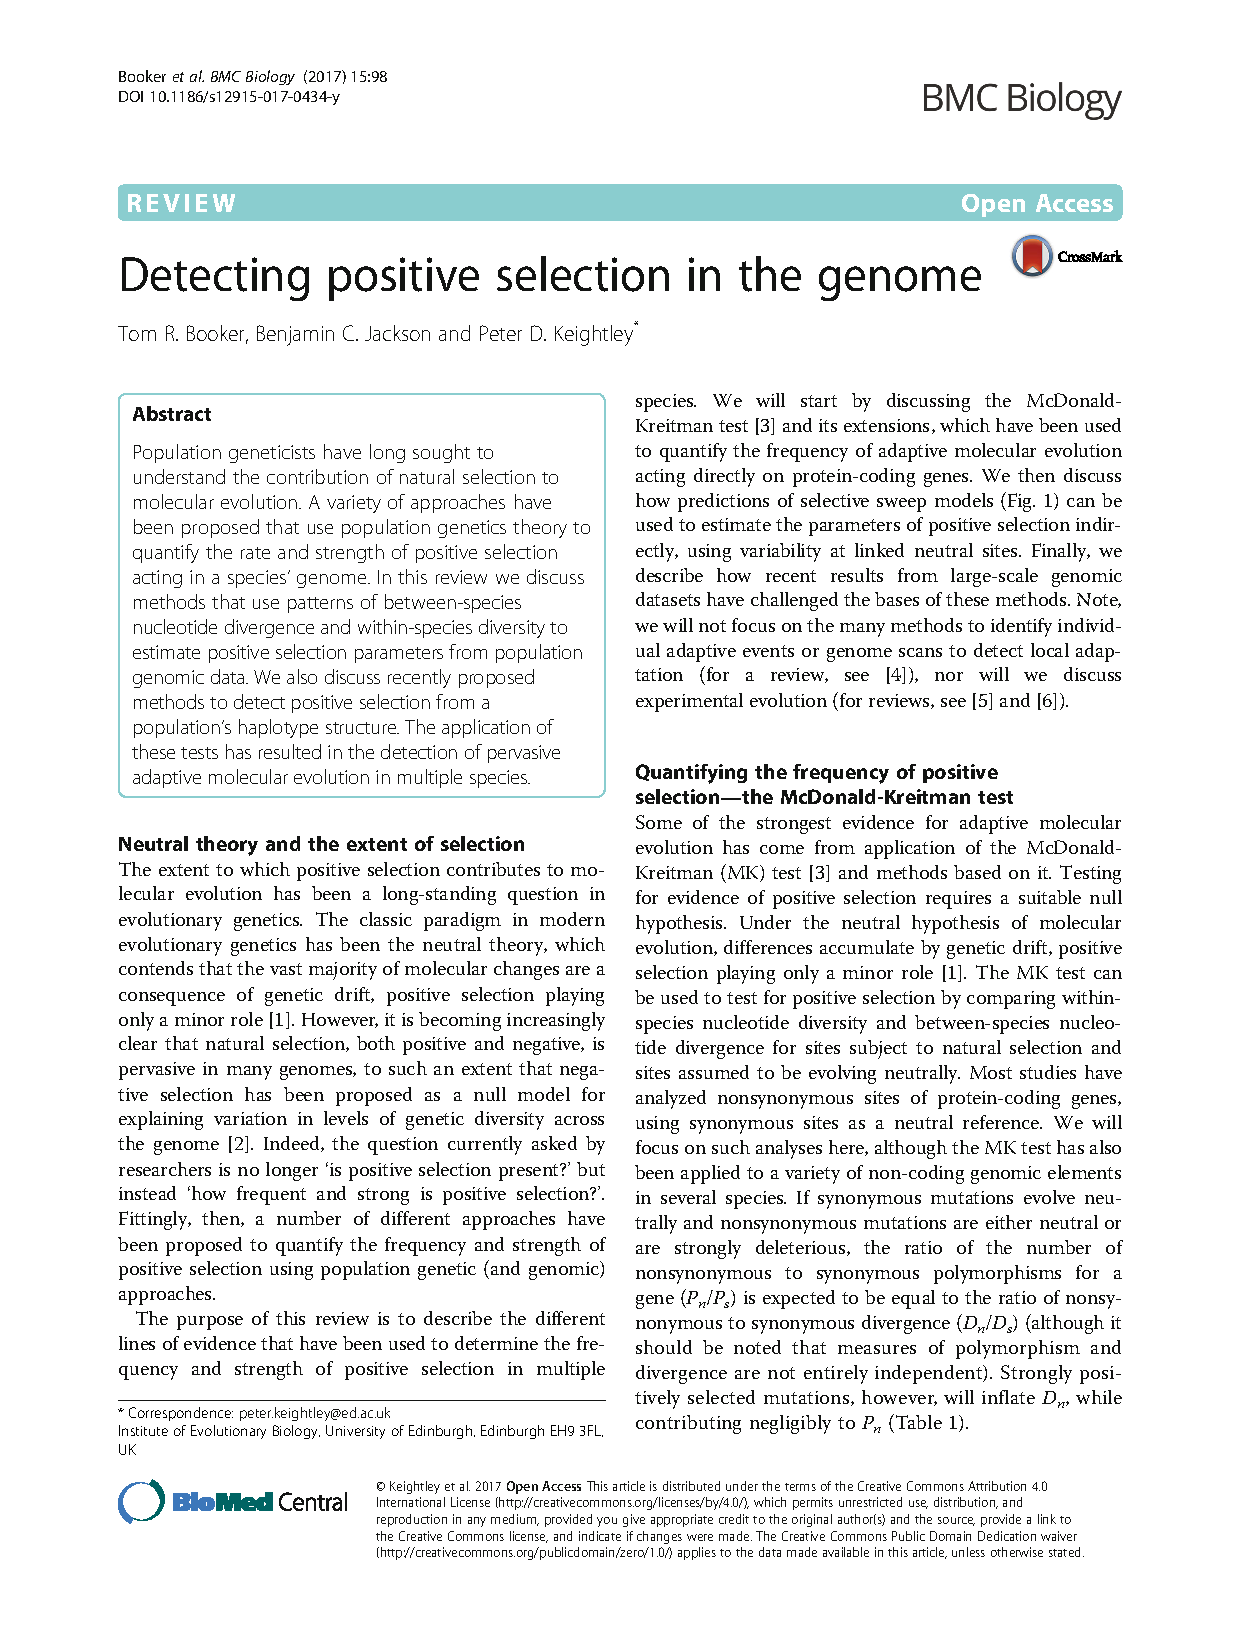
\includepdf[pages=-, scale = 0.8 , pagecommand={\pagestyle{fancy}}]{/Users/s0784966/Dropbox/Thesis/chapter1Appendix/Booker_et_al_2017_REVIEW.pdf}

		\chapter{Recombination in wild mice}

		
\section{Supplementary Material}
Included here are the supplementary figures and tables for Chapter 2.
\linespread{1}
\begin{table}[h!]
\centering
\caption[Comparison of the fit of demographic models based on the analysis of 4-fold sites and CNE-flanks in \textit{M. m. castaneus}]{Comparison of the fit of demographic models based on the analysis of 4-fold sites and CNE-flanks in \textit{M. m. castaneus}.}
 \begin{tabular}{c c c c c } 

\toprule
       &Epochs&$\Delta lnL$& $\chi^2$& \# Estimated Parameters \\ \hline
\multirow{3}{*}{4-fold} & 	1 &	1,620	 &	22,500 	&	2 \\
		 &	2 &	159		 &	2,930 	&	4 \\
 		&	3 &	0.0		 &	553 		&	6 \\ \hdashline
\multirow{3}{*}{CNE-flank} &	1 &	19,100	 &	53,500 	&	2 \\
		 &	2 &	1,350	 &	5,070	&	4 \\
 		&	3 &	0.0 		 &	975 		&	6 \\
\bottomrule
\end{tabular}
\label{tab:CS1}
\end{table}

\begin{table}[h!]
\centering
\caption[Parameters of the best-fitting demographic model estimated from the analysis of 4-fold and CNE-flanking sites]{Parameters of the best-fitting demographic model estimated from the analysis of 4-fold and CNE-flanking sites. }
 \begin{tabular}{c c c c c } 

\toprule
	&4-fold	&CNE-flank \\ \hline
N2/N1&	0.40&	0.07 \\
t2/N1&	0.44&	0.17 \\
N3/N1&	0.40&	1.00 \\
t3/N1&	1.10&	0.63 \\
\bottomrule

\end{tabular}
\label{tab:C3S2}
\end{table}
\begin{table}[h!]
\centering
\caption[Parameters of the 3-epoch demographic model at different sample sizes]{Parameters of the 3-epoch demographic model at different sample sizes. Down sampled datasets were generated by randomly selecting alleles, with respect to frequency, from the full dataset of 10 individuals.}
 \begin{tabular}{c c c c c } 

\toprule
\multirow{2}{*}{Parameter} & \multicolumn{3}{c}{Number of alleles sampled} \\ 
	&	$n = 10$ & 	$n = 16$ & 	$n = 20$ \\ \hline
N2/N1 &	0.030 &	0.030 &	0.060 \\
t2/N1 &	0.204 &	0.140 &	0.181 \\
N3/N1 &	0.120 &	0.200 &	0.800 \\
t3/N1 &	0.080 &	0.220 &	0.461 \\
\bottomrule

\end{tabular}
\label{tab:C3S3}
\end{table}
\begin{table}[h!]
\centering
\caption[Likelihood differences between models of the dDFE fitted with or without a single class of adaptive mutations]{Likelihood differences between models of the deleterious DFE (dDFE) fitted with or without a single class of adaptive mutations.}
 \begin{tabular}{c c c c } 

\toprule
\multirow{2}{*}{\textbf{Site Type}} 	& \multirow{2}{*}{\textbf{dDFE Model}}& 	\multicolumn{2}{c}{\textbf{$\Delta lnL$}} \\
    &  &   \textbf{dDFE}	 & \textbf{dDFE + Adaptive Mutations} \\ \hline
\multirow{2}{*}{\textbf{0-fold}} &	1-Class	&49,300	&4.18 \\
	   &2-Class	&129 	&0.00 \\
	   &3-Class	&129	    &0.00 \\
	   &Gamma	&247	 	&4.18 \\ \hdashline
\multirow{2}{*}{\textbf{CNE}}	   &1-Class	&51,000	&245 \\
	   &2-Class	&1,660	&3.41 \\
	   &3-Class	&1,480	&0.00 \\
	   &Gamma	&2,310	&19.3 \\ \hdashline
\multirow{2}{*}{\textbf{UTR}}	   &1-Class	&6,170	&32.7 \\
	   &2-Class	&335	    &0.00 \\
	   &3-Class	&335	    &0.00 \\
	   &Gamma	&970	    &13.5 \\
\bottomrule

\end{tabular}
\label{tab:C3S4}
\end{table}
 
 \begin{figure}
   \centering      
   \noindent\makebox[\textwidth]{\includegraphics[width=\textwidth]{/Users/s0784966/Dropbox/Thesis/chapter2Appendix/Figures/FigureS1.pdf}}
 \caption[]{}
 \label{fig:1}
\end{figure}

 
 \begin{figure}
   \centering      
   \noindent\makebox[\textwidth]{\includegraphics[width=\textwidth]{/Users/s0784966/Dropbox/Thesis/chapter2Appendix/Figures/FigureS2.pdf}}
 \caption[The effect of switch errors on recombination rate inference]{The effect of switch errors on the mean recombination rate inferred using LDhelmet with a block penalty of 100. Each black point represents results for a window of 4000 SNPs, with 200 SNPs overlapping between adjacent windows, using sequences simulated in SLiM for a constant value of $\rho/bp$. Red points are mean values. Switch errors were randomly incorporated at heterozygous SNPs with probability 0.0046. The dotted line shows the value when the inferred and true rates are equal}
 \label{fig:1}
\end{figure}

 
 \begin{figure}
   \centering      
   \noindent\makebox[\textwidth]{\includegraphics[width=\textwidth]{/Users/s0784966/Dropbox/Thesis/chapter2Appendix/Figures/FigureS3.pdf}}
 \caption[The effect of switch errors on recombination rate inference]{The effect of switch errors on the mean recombination rate inferred using LDhelmet with a block penalty of 100. Each black point represents results for a window of 4000 SNPs, with 200 SNPs overlapping between adjacent windows, using sequences simulated in SLiM for a constant value of $\rho/bp$. Red points are mean values. Switch errors were randomly incorporated at heterozygous SNPs with probability 0.0046. The dotted line shows the value when the inferred and true rates are equal}
 \label{fig:1}
\end{figure}

\linespread{2}
\pagebreak
\section{Booker \emph{et al.} 2017 - Genetics}
\includepdf[pages=-, scale = 0.8 , pagecommand={\pagestyle{fancy}}]{/Users/s0784966/Dropbox/Thesis/chapter2Appendix/Booker_et_al2017_Genetics.pdf}

	\end{appendices}


\end{document}